% Options for packages loaded elsewhere
\PassOptionsToPackage{unicode}{hyperref}
\PassOptionsToPackage{hyphens}{url}
%
\documentclass[
  ignorenonframetext,
]{beamer}
\usepackage{pgfpages}
\setbeamertemplate{caption}[numbered]
\setbeamertemplate{caption label separator}{: }
\setbeamercolor{caption name}{fg=normal text.fg}
\beamertemplatenavigationsymbolsempty
% Prevent slide breaks in the middle of a paragraph
\widowpenalties 1 10000
\raggedbottom
\setbeamertemplate{part page}{
  \centering
  \begin{beamercolorbox}[sep=16pt,center]{part title}
    \usebeamerfont{part title}\insertpart\par
  \end{beamercolorbox}
}
\setbeamertemplate{section page}{
  \centering
  \begin{beamercolorbox}[sep=12pt,center]{part title}
    \usebeamerfont{section title}\insertsection\par
  \end{beamercolorbox}
}
\setbeamertemplate{subsection page}{
  \centering
  \begin{beamercolorbox}[sep=8pt,center]{part title}
    \usebeamerfont{subsection title}\insertsubsection\par
  \end{beamercolorbox}
}
\AtBeginPart{
  \frame{\partpage}
}
\AtBeginSection{
  \ifbibliography
  \else
    \frame{\sectionpage}
  \fi
}
\AtBeginSubsection{
  \frame{\subsectionpage}
}
\usepackage{amsmath,amssymb}
\usepackage{iftex}
\ifPDFTeX
  \usepackage[T1]{fontenc}
  \usepackage[utf8]{inputenc}
  \usepackage{textcomp} % provide euro and other symbols
\else % if luatex or xetex
  \usepackage{unicode-math} % this also loads fontspec
  \defaultfontfeatures{Scale=MatchLowercase}
  \defaultfontfeatures[\rmfamily]{Ligatures=TeX,Scale=1}
\fi
\usepackage{lmodern}
\usetheme[]{Madrid}
\ifPDFTeX\else
  % xetex/luatex font selection
\fi
% Use upquote if available, for straight quotes in verbatim environments
\IfFileExists{upquote.sty}{\usepackage{upquote}}{}
\IfFileExists{microtype.sty}{% use microtype if available
  \usepackage[]{microtype}
  \UseMicrotypeSet[protrusion]{basicmath} % disable protrusion for tt fonts
}{}
\makeatletter
\@ifundefined{KOMAClassName}{% if non-KOMA class
  \IfFileExists{parskip.sty}{%
    \usepackage{parskip}
  }{% else
    \setlength{\parindent}{0pt}
    \setlength{\parskip}{6pt plus 2pt minus 1pt}}
}{% if KOMA class
  \KOMAoptions{parskip=half}}
\makeatother
\usepackage{xcolor}
\newif\ifbibliography
\usepackage{color}
\usepackage{fancyvrb}
\newcommand{\VerbBar}{|}
\newcommand{\VERB}{\Verb[commandchars=\\\{\}]}
\DefineVerbatimEnvironment{Highlighting}{Verbatim}{commandchars=\\\{\}}
% Add ',fontsize=\small' for more characters per line
\usepackage{framed}
\definecolor{shadecolor}{RGB}{248,248,248}
\newenvironment{Shaded}{\begin{snugshade}}{\end{snugshade}}
\newcommand{\AlertTok}[1]{\textcolor[rgb]{0.94,0.16,0.16}{#1}}
\newcommand{\AnnotationTok}[1]{\textcolor[rgb]{0.56,0.35,0.01}{\textbf{\textit{#1}}}}
\newcommand{\AttributeTok}[1]{\textcolor[rgb]{0.13,0.29,0.53}{#1}}
\newcommand{\BaseNTok}[1]{\textcolor[rgb]{0.00,0.00,0.81}{#1}}
\newcommand{\BuiltInTok}[1]{#1}
\newcommand{\CharTok}[1]{\textcolor[rgb]{0.31,0.60,0.02}{#1}}
\newcommand{\CommentTok}[1]{\textcolor[rgb]{0.56,0.35,0.01}{\textit{#1}}}
\newcommand{\CommentVarTok}[1]{\textcolor[rgb]{0.56,0.35,0.01}{\textbf{\textit{#1}}}}
\newcommand{\ConstantTok}[1]{\textcolor[rgb]{0.56,0.35,0.01}{#1}}
\newcommand{\ControlFlowTok}[1]{\textcolor[rgb]{0.13,0.29,0.53}{\textbf{#1}}}
\newcommand{\DataTypeTok}[1]{\textcolor[rgb]{0.13,0.29,0.53}{#1}}
\newcommand{\DecValTok}[1]{\textcolor[rgb]{0.00,0.00,0.81}{#1}}
\newcommand{\DocumentationTok}[1]{\textcolor[rgb]{0.56,0.35,0.01}{\textbf{\textit{#1}}}}
\newcommand{\ErrorTok}[1]{\textcolor[rgb]{0.64,0.00,0.00}{\textbf{#1}}}
\newcommand{\ExtensionTok}[1]{#1}
\newcommand{\FloatTok}[1]{\textcolor[rgb]{0.00,0.00,0.81}{#1}}
\newcommand{\FunctionTok}[1]{\textcolor[rgb]{0.13,0.29,0.53}{\textbf{#1}}}
\newcommand{\ImportTok}[1]{#1}
\newcommand{\InformationTok}[1]{\textcolor[rgb]{0.56,0.35,0.01}{\textbf{\textit{#1}}}}
\newcommand{\KeywordTok}[1]{\textcolor[rgb]{0.13,0.29,0.53}{\textbf{#1}}}
\newcommand{\NormalTok}[1]{#1}
\newcommand{\OperatorTok}[1]{\textcolor[rgb]{0.81,0.36,0.00}{\textbf{#1}}}
\newcommand{\OtherTok}[1]{\textcolor[rgb]{0.56,0.35,0.01}{#1}}
\newcommand{\PreprocessorTok}[1]{\textcolor[rgb]{0.56,0.35,0.01}{\textit{#1}}}
\newcommand{\RegionMarkerTok}[1]{#1}
\newcommand{\SpecialCharTok}[1]{\textcolor[rgb]{0.81,0.36,0.00}{\textbf{#1}}}
\newcommand{\SpecialStringTok}[1]{\textcolor[rgb]{0.31,0.60,0.02}{#1}}
\newcommand{\StringTok}[1]{\textcolor[rgb]{0.31,0.60,0.02}{#1}}
\newcommand{\VariableTok}[1]{\textcolor[rgb]{0.00,0.00,0.00}{#1}}
\newcommand{\VerbatimStringTok}[1]{\textcolor[rgb]{0.31,0.60,0.02}{#1}}
\newcommand{\WarningTok}[1]{\textcolor[rgb]{0.56,0.35,0.01}{\textbf{\textit{#1}}}}
\usepackage{graphicx}
\makeatletter
\def\maxwidth{\ifdim\Gin@nat@width>\linewidth\linewidth\else\Gin@nat@width\fi}
\def\maxheight{\ifdim\Gin@nat@height>\textheight\textheight\else\Gin@nat@height\fi}
\makeatother
% Scale images if necessary, so that they will not overflow the page
% margins by default, and it is still possible to overwrite the defaults
% using explicit options in \includegraphics[width, height, ...]{}
\setkeys{Gin}{width=\maxwidth,height=\maxheight,keepaspectratio}
% Set default figure placement to htbp
\makeatletter
\def\fps@figure{htbp}
\makeatother
\setlength{\emergencystretch}{3em} % prevent overfull lines
\providecommand{\tightlist}{%
  \setlength{\itemsep}{0pt}\setlength{\parskip}{0pt}}
\setcounter{secnumdepth}{-\maxdimen} % remove section numbering
\logo{
\includegraphics[height=1cm,width=3cm]{logo.png}}
\usetheme{Madrid}
\usefonttheme{serif}
\setbeamertemplate{navigation symbols}{}
\usepackage{lmodern}  % for bold teletype font
\usepackage{amsmath}  % for \hookrightarrow
\usepackage{xcolor}   % for \textcolor


\ifLuaTeX
  \usepackage{selnolig}  % disable illegal ligatures
\fi
\IfFileExists{bookmark.sty}{\usepackage{bookmark}}{\usepackage{hyperref}}
\IfFileExists{xurl.sty}{\usepackage{xurl}}{} % add URL line breaks if available
\urlstyle{same}
\hypersetup{
  pdftitle={Leksioni 8},
  pdfauthor={Endri Raco},
  hidelinks,
  pdfcreator={LaTeX via pandoc}}

\title{Leksioni 8}
\author{Endri Raco}
\date{05 May, 2024}

\begin{document}
\frame{\titlepage}

\begin{frame}[allowframebreaks]
  \tableofcontents[hideallsubsections]
\end{frame}
\hypertarget{tuxeb-dhuxebnat-raster-vazhdim}{%
\section{Të dhënat Raster
(vazhdim)}\label{tuxeb-dhuxebnat-raster-vazhdim}}

\begin{frame}[fragile]{Analiza e Pikave dhe Vlerësimi i Dendësisë së
Kernelit (KDE)}
\protect\hypertarget{analiza-e-pikave-dhe-vleruxebsimi-i-denduxebsisuxeb-suxeb-kernelit-kde}{}
\AddToHookNext{env/Highlighting/begin}{\tiny}

\begin{Shaded}
\begin{Highlighting}[]
\ImportTok{import}\NormalTok{ urllib.request}

\CommentTok{\# Shkarkoni të dhënat e anijeve të mbytura historike}
\NormalTok{url\_shipwrecks }\OperatorTok{=} \StringTok{\textquotesingle{}https://github.com/endri81/instatgis/blob/master/data/gis4/darmc\_historical\_shipwrecks\_500bce\_1500ce.geojson?raw=true\textquotesingle{}}
\NormalTok{file\_name\_shipwrecks }\OperatorTok{=} \StringTok{\textquotesingle{}data/darmc\_historical\_shipwrecks\_500bce\_1500ce.geojson\textquotesingle{}}
\NormalTok{urllib.request.urlretrieve(url\_shipwrecks, file\_name\_shipwrecks)}

\CommentTok{\# Shkarkoni gjithashtu kufijtë e vendeve}
\NormalTok{url\_boundaries }\OperatorTok{=} \StringTok{\textquotesingle{}https://github.com/endri81/instatgis/blob/master/data/gis4/natural\_earth\_world\_boundaries\_50m\_2018.geojson?raw=true\textquotesingle{}}
\NormalTok{file\_name\_boundaries }\OperatorTok{=} \StringTok{\textquotesingle{}data/natural\_earth\_world\_boundaries\_50m\_2018.geojson\textquotesingle{}}
\NormalTok{urllib.request.urlretrieve(url\_boundaries, file\_name\_boundaries)}
\end{Highlighting}
\end{Shaded}
\end{frame}

\begin{frame}[fragile]{Ngarkimi dhe Projekti i Dataset-eve}
\protect\hypertarget{ngarkimi-dhe-projekti-i-dataset-eve}{}
\AddToHookNext{env/Highlighting/begin}{\tiny}

\begin{Shaded}
\begin{Highlighting}[]
\ImportTok{import}\NormalTok{ geopandas }\ImportTok{as}\NormalTok{ gpd}

\CommentTok{\# Ngarkoni dataset{-}in dhe projektoni në 3035 (Lambert, i përshtatshëm për Evropën)}
\NormalTok{ship\_df }\OperatorTok{=}\NormalTok{ gpd.read\_file(}\StringTok{\textquotesingle{}data/darmc\_historical\_shipwrecks\_500bce\_1500ce.geojson\textquotesingle{}}\NormalTok{).to\_crs(}\DecValTok{3035}\NormalTok{)}
\NormalTok{countries\_df }\OperatorTok{=}\NormalTok{ gpd.read\_file(}\StringTok{\textquotesingle{}data/natural\_earth\_world\_boundaries\_50m\_2018.geojson\textquotesingle{}}\NormalTok{).to\_crs(}\DecValTok{3035}\NormalTok{)}
\end{Highlighting}
\end{Shaded}
\end{frame}

\begin{frame}[fragile]{Shfaqni një shembull të të dhënave}
\protect\hypertarget{shfaqni-njuxeb-shembull-tuxeb-tuxeb-dhuxebnave}{}
\AddToHookNext{env/Highlighting/begin}{\tiny}

\begin{Shaded}
\begin{Highlighting}[]
\NormalTok{ship\_df.sample(}\DecValTok{5}\NormalTok{)}
\end{Highlighting}
\end{Shaded}
\end{frame}

\begin{frame}{Shfaqni një shembull të të dhënave}
\protect\hypertarget{shfaqni-njuxeb-shembull-tuxeb-tuxeb-dhuxebnave-1}{}
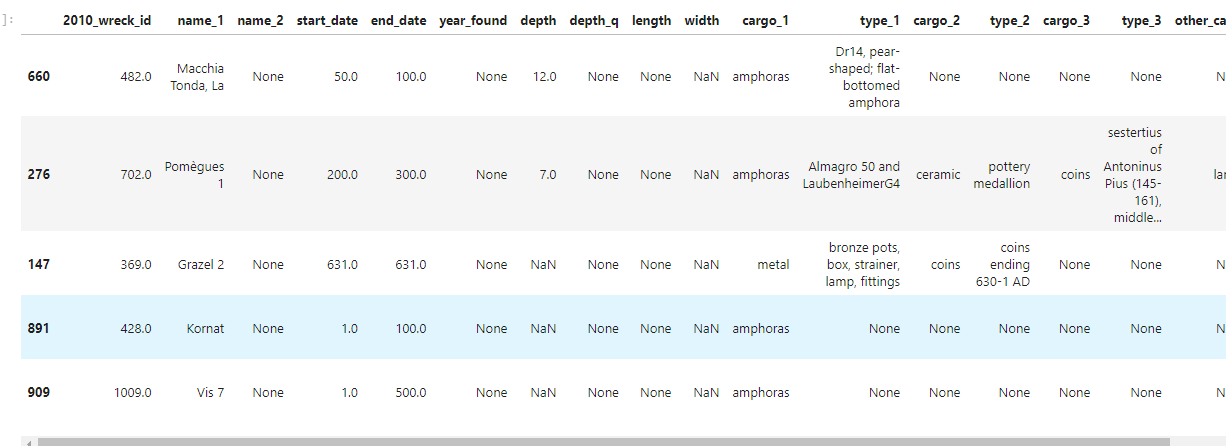
\includegraphics{./Figs/ship.png}
\end{frame}

\begin{frame}[fragile]{Vizualizimi i Pikave}
\protect\hypertarget{vizualizimi-i-pikave}{}
\AddToHookNext{env/Highlighting/begin}{\tiny}

\begin{Shaded}
\begin{Highlighting}[]
\ImportTok{import}\NormalTok{ geoplot}
\ImportTok{import}\NormalTok{ matplotlib.pyplot }\ImportTok{as}\NormalTok{ plt}

\CommentTok{\# Përkufizoni kanavacën}
\NormalTok{f, ax }\OperatorTok{=}\NormalTok{ plt.subplots(figsize}\OperatorTok{=}\NormalTok{(}\DecValTok{10}\NormalTok{,}\DecValTok{7}\NormalTok{))}

\CommentTok{\# Vizualizoni dy shtresa}
\NormalTok{countries\_df.plot(ax}\OperatorTok{=}\NormalTok{ax, color}\OperatorTok{=}\StringTok{\textquotesingle{}lightgray\textquotesingle{}}\NormalTok{, edgecolor}\OperatorTok{=}\StringTok{"none"}\NormalTok{, linewidth}\OperatorTok{=}\FloatTok{.5}\NormalTok{)}
\NormalTok{geoplot.pointplot(ship\_df, s}\OperatorTok{=}\DecValTok{2}\NormalTok{, color}\OperatorTok{=}\StringTok{\textquotesingle{}red\textquotesingle{}}\NormalTok{, ax}\OperatorTok{=}\NormalTok{ax, alpha}\OperatorTok{=}\FloatTok{.1}\NormalTok{)}

\CommentTok{\# Vendosni kufijtë e hartës}
\CommentTok{\# Krijoni një buffer për të shtuar një margjinë}
\NormalTok{buff }\OperatorTok{=}\NormalTok{ ship\_df.}\BuiltInTok{buffer}\NormalTok{(}\DecValTok{1}\NormalTok{)}
\NormalTok{xlim }\OperatorTok{=}\NormalTok{ ([buff.total\_bounds[}\DecValTok{0}\NormalTok{], buff.total\_bounds[}\DecValTok{2}\NormalTok{]])}
\NormalTok{ylim }\OperatorTok{=}\NormalTok{ ([buff.total\_bounds[}\DecValTok{1}\NormalTok{], buff.total\_bounds[}\DecValTok{3}\NormalTok{]])}
\NormalTok{ax.set\_xlim(xlim)}
\NormalTok{ax.set\_ylim(ylim)}

\CommentTok{\# Vendosni titullin e hartës}
\NormalTok{ax.set\_title(}\StringTok{\textquotesingle{}Anije të Mbytura (500 p.e.s. {-} 1500 e.s.)\textquotesingle{}}\NormalTok{)}

\CommentTok{\# Shfaqni rezultatet}
\NormalTok{plt.show()}
\end{Highlighting}
\end{Shaded}
\end{frame}

\begin{frame}{Vizualizimi i Pikave}
\protect\hypertarget{vizualizimi-i-pikave-1}{}
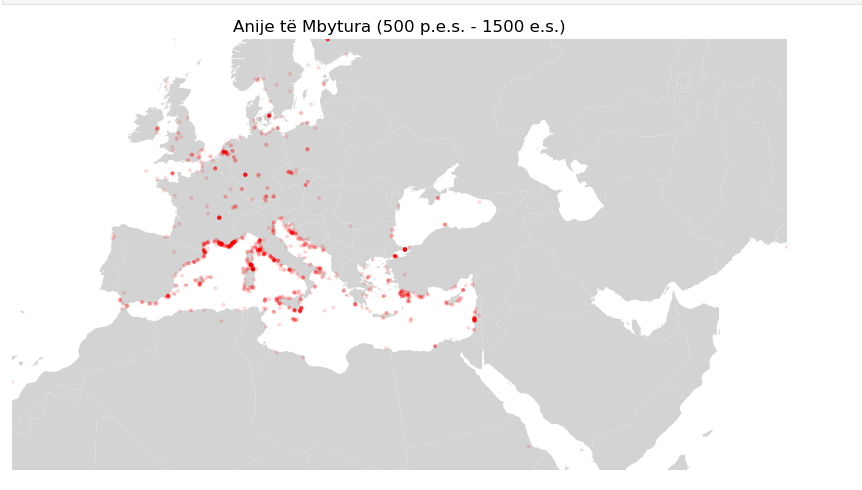
\includegraphics{./Figs/anije.png}
\end{frame}

\begin{frame}{Histogram 2D}
\protect\hypertarget{histogram-2d}{}
\begin{itemize}
\tightlist
\item
  Një mënyrë më e mirë për të përfaqësuar një densitet hapësinor është
  një histogram dy-dimensional (hist2d), i njohur gjithashtu si një
  grafik rrjeti.
\end{itemize}
\end{frame}

\begin{frame}{Histogram 2D}
\protect\hypertarget{histogram-2d-1}{}
\begin{itemize}
\tightlist
\item
  Vini re se një nga avantazhet e Python është mundësia e ndryshimit të
  parametrave të një funksioni përmes një cikli for (për shembull, numri
  i shtyllave në një histogram) dhe krahasimi i rezultateve.
\end{itemize}
\end{frame}

\begin{frame}[fragile]{Histogram 2D}
\protect\hypertarget{histogram-2d-2}{}
\AddToHookNext{env/Highlighting/begin}{\tiny}

\begin{Shaded}
\begin{Highlighting}[]
\CommentTok{\# riprojektojmë në lon/lat për të pasur koordinata më të interpretueshme}
\NormalTok{ship\_df }\OperatorTok{=}\NormalTok{ ship\_df.to\_crs(}\DecValTok{4326}\NormalTok{)}

\CommentTok{\# le të luajmë me numrin e bins:}
\ControlFlowTok{for}\NormalTok{ bin\_n }\KeywordTok{in}\NormalTok{ [}\DecValTok{10}\NormalTok{,}\DecValTok{20}\NormalTok{,}\DecValTok{30}\NormalTok{,}\DecValTok{40}\NormalTok{]:}
    \BuiltInTok{print}\NormalTok{(}\StringTok{"bin\_n"}\NormalTok{,bin\_n)}
\NormalTok{    h }\OperatorTok{=}\NormalTok{ plt.hist2d(ship\_df.geometry.x, ship\_df.geometry.y, bins}\OperatorTok{=}\NormalTok{bin\_n, density}\OperatorTok{=}\VariableTok{False}\NormalTok{)}
\NormalTok{    plt.colorbar(h[}\DecValTok{3}\NormalTok{])}
\NormalTok{    plt.title(}\StringTok{\textquotesingle{}2D histograma e anijeve (bins=\textquotesingle{}}\OperatorTok{+}\BuiltInTok{str}\NormalTok{(bin\_n)}\OperatorTok{+}\StringTok{")"}\NormalTok{)}
\NormalTok{    plt.show()}
\end{Highlighting}
\end{Shaded}
\end{frame}

\begin{frame}{Histogram 2D}
\protect\hypertarget{histogram-2d-3}{}
Këto grafikë tregojnë praninë e një zone me densitet jashtëzakonisht të
lartë midis Francës, Korsikës dhe Italisë:
\end{frame}

\begin{frame}{Grafiku KDE}
\protect\hypertarget{grafiku-kde}{}
\begin{itemize}
\item
  Një qasje më shkencore është vlerësimi i densitetit të bërthamës
  (KDE).
\item
  \textbf{geoplot.kdeplot(\ldots)} mund të vizatojë një KDE duke u nisur
  nga të dhënat e pikës.
\end{itemize}
\end{frame}

\begin{frame}{Grafiku KDE}
\protect\hypertarget{grafiku-kde-1}{}
\begin{itemize}
\tightlist
\item
  Një parametër vendimtar është \textbf{bandwidth} (bw), që është pragu
  i distancës që përdoret për të prodhuar sipërfaqen (distancat më të
  shkurtra rezultojnë në një sipërfaqe më të detajuar):
\end{itemize}
\end{frame}

\begin{frame}[fragile]{Grafiku KDE}
\protect\hypertarget{grafiku-kde-2}{}
\AddToHookNext{env/Highlighting/begin}{\tiny}

\begin{Shaded}
\begin{Highlighting}[]
\CommentTok{\# transformojmë në lon/lat}
\NormalTok{ship\_df\_ll }\OperatorTok{=}\NormalTok{ ship\_df.to\_crs(}\DecValTok{4326}\NormalTok{)}

\CommentTok{\# gjenerojmë KDE me bandwidth të ndryshëm}
\ControlFlowTok{for}\NormalTok{ bandwidth }\KeywordTok{in}\NormalTok{ [}\FloatTok{.1}\NormalTok{, }\FloatTok{.2}\NormalTok{, }\FloatTok{.3}\NormalTok{, }\FloatTok{.4}\NormalTok{]:}
    \BuiltInTok{print}\NormalTok{(}\StringTok{"bandwidth:"}\NormalTok{,bandwidth)}
    \CommentTok{\# konturet e KDE}
\NormalTok{    ax }\OperatorTok{=}\NormalTok{ geoplot.kdeplot(ship\_df\_ll, shade}\OperatorTok{=}\VariableTok{False}\NormalTok{, bw}\OperatorTok{=}\NormalTok{bandwidth, figsize}\OperatorTok{=}\NormalTok{(}\DecValTok{12}\NormalTok{, }\DecValTok{12}\NormalTok{), alpha}\OperatorTok{=}\FloatTok{.5}\NormalTok{)}
    \CommentTok{\# shtojmë vijën bregdetare}
\NormalTok{    countries\_df.to\_crs(}\DecValTok{4326}\NormalTok{).plot(ax}\OperatorTok{=}\NormalTok{ax, color}\OperatorTok{=}\StringTok{\textquotesingle{}lightgray\textquotesingle{}}\NormalTok{, edgecolor}\OperatorTok{=}\StringTok{"none"}\NormalTok{, linewidth}\OperatorTok{=}\FloatTok{.5}\NormalTok{)}
    \CommentTok{\# shtojmë titull}
\NormalTok{    plt.title(}\StringTok{\textquotesingle{}Dendësia e mbytjeve të anijeve (KDE, bw=\textquotesingle{}}\OperatorTok{+}\BuiltInTok{str}\NormalTok{(bandwidth)}\OperatorTok{+}\StringTok{")"}\NormalTok{, fontsize}\OperatorTok{=}\DecValTok{18}\NormalTok{)}
    \CommentTok{\# figura}
\NormalTok{    plt.show()}
\end{Highlighting}
\end{Shaded}
\end{frame}

\begin{frame}{Grafiku KDE}
\protect\hypertarget{grafiku-kde-3}{}
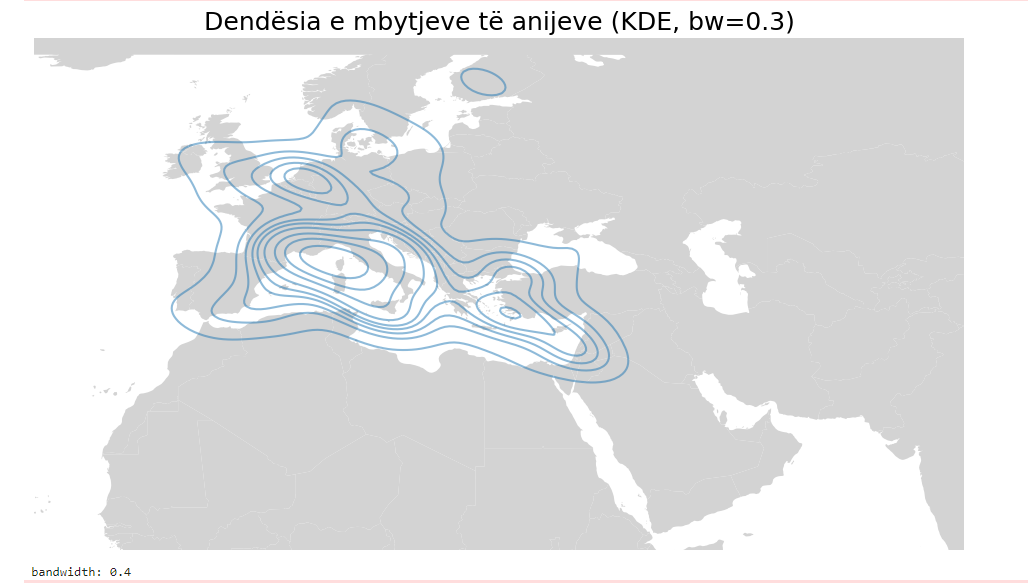
\includegraphics{./Figs/kde.png}
\end{frame}

\begin{frame}{Analiza e të dhënave}
\protect\hypertarget{analiza-e-tuxeb-dhuxebnave}{}
\begin{itemize}
\item
  Këta grafikë KDE tregojnë se dataset-i ka një përqendrim shumë të
  lartë të pikave në Detin Mesdhe, midis Francës Jugore, Korsikës dhe
  Bregut Perëndimor të Italisë.
\item
  Në të gjitha grafikët, kjo qendër graviteti shfaqet qartë.
\end{itemize}
\end{frame}

\begin{frame}{Analiza e të dhënave}
\protect\hypertarget{analiza-e-tuxeb-dhuxebnave-1}{}
\begin{itemize}
\tightlist
\item
  Në aspektin shkencor, kjo mund të tregojë se kishte shumë më tepër
  mbytje anijesh aty se gjetkë, ose (më e mundshme) që të dhënat
  historike janë më të pasura dhe më të hollësishme për atë zonë.
\end{itemize}
\end{frame}

\hypertarget{algjebra-e-hartave}{%
\section{Algjebra e Hartave}\label{algjebra-e-hartave}}

\begin{frame}{Algjebra e Hartave}
\protect\hypertarget{algjebra-e-hartave-1}{}
\begin{itemize}
\item
  Termi ``algjebra e hartave'' i referohet idesë së aplikimit të
  operacioneve algjebrike në dataset-e raster.
\item
  Për shembull, mund të dëshirojmë të zbresim nga njëri- tjetri dy
  rastera të temperaturës të kapur në kohë të ndryshme për të vëzhguar
  ndryshimin e temperaturës:
\end{itemize}
\end{frame}

\begin{frame}{Algjebra e Hartave}
\protect\hypertarget{algjebra-e-hartave-2}{}
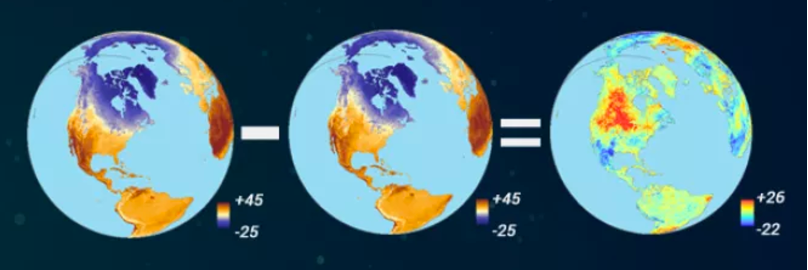
\includegraphics{./Figs/map_algebra1.png}
\end{frame}

\begin{frame}{Algjebra e Hartave}
\protect\hypertarget{algjebra-e-hartave-3}{}
Në praktikë, ky është një operacion aritmetik i aplikuar në çdo qelizë
të të dy raster-ve:

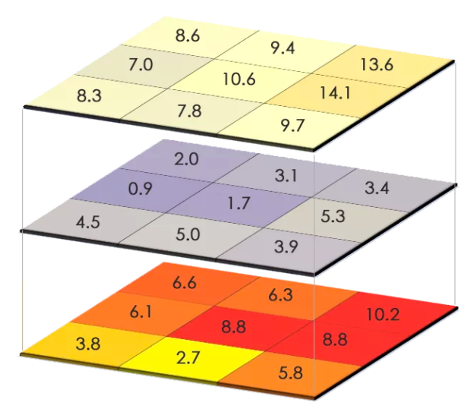
\includegraphics{./Figs/map_algebra2.png}
\end{frame}

\begin{frame}{Algjebra e hartave në Python}
\protect\hypertarget{algjebra-e-hartave-nuxeb-python}{}
\begin{itemize}
\item
  Kur aksesojmë raster me \textbf{rasterio} ose \textbf{gdal}, ne mund
  të kryejmë çdo lloj llogaritjeje algjebrike lineare mbi të dhënat duke
  përdorur \textbf{numpy, scipy} dhe shumë paketa të tjera të fuqishme
  të Python.
\item
  Statistikat zonale suportohen në librarinë \textbf{rasterstats}.
\end{itemize}
\end{frame}

\begin{frame}{Algjebra e hartave në Python}
\protect\hypertarget{algjebra-e-hartave-nuxeb-python-1}{}
\begin{itemize}
\tightlist
\item
  Kjo është arsyeja kryesore pse Python përdoret gjerësisht në
  komunitetet e remote sensing, machine learning, dhe AI.
\end{itemize}
\end{frame}

\begin{frame}{Ngarkoni të dhënat e temperaturës}
\protect\hypertarget{ngarkoni-tuxeb-dhuxebnat-e-temperaturuxebs}{}
\begin{itemize}
\tightlist
\item
  Si një shembull, le të shkarkojmë dhe vizualizojmë dy datasete raster
  që përfaqësojnë temperaturën mesatare në vitin 2000 dhe 2017.
\end{itemize}
\end{frame}

\begin{frame}[fragile]{Ngarkoni të dhënat e temperaturës}
\protect\hypertarget{ngarkoni-tuxeb-dhuxebnat-e-temperaturuxebs-1}{}
\AddToHookNext{env/Highlighting/begin}{\tiny}

\begin{Shaded}
\begin{Highlighting}[]
\ImportTok{import}\NormalTok{ urllib.request}

\CommentTok{\# Define new URLs and file names}
\NormalTok{url\_2000 }\OperatorTok{=} \StringTok{"https://github.com/endri81/instatgis/blob/master/data/gis4/air\_temp\_2000{-}average.tif?raw=true"}
\NormalTok{url\_2017 }\OperatorTok{=} \StringTok{"https://github.com/endri81/instatgis/blob/master/data/gis4/air\_temp\_2017{-}average.tif?raw=true"}
\NormalTok{file\_name\_2000 }\OperatorTok{=} \StringTok{\textquotesingle{}data/air\_temp\_2000{-}average.tif\textquotesingle{}}
\NormalTok{file\_name\_2017 }\OperatorTok{=} \StringTok{\textquotesingle{}data/air\_temp\_2017{-}average.tif\textquotesingle{}}

\CommentTok{\# Download the files}
\NormalTok{urllib.request.urlretrieve(url\_2000, file\_name\_2000)}
\NormalTok{urllib.request.urlretrieve(url\_2017, file\_name\_2017)}
\end{Highlighting}
\end{Shaded}
\end{frame}

\begin{frame}[fragile]{Ngarkoni të dhënat e temperaturës}
\protect\hypertarget{ngarkoni-tuxeb-dhuxebnat-e-temperaturuxebs-2}{}
\AddToHookNext{env/Highlighting/begin}{\tiny}

\begin{Shaded}
\begin{Highlighting}[]
\NormalTok{temp00 }\OperatorTok{=}\NormalTok{ rasterio.}\BuiltInTok{open}\NormalTok{(}\StringTok{\textquotesingle{}data/air\_temp\_2000{-}average.tif\textquotesingle{}}\NormalTok{)}
\BuiltInTok{print}\NormalTok{(temp00.meta)}
\NormalTok{temp17 }\OperatorTok{=}\NormalTok{ rasterio.}\BuiltInTok{open}\NormalTok{(}\StringTok{\textquotesingle{}data/air\_temp\_2017{-}average.tif\textquotesingle{}}\NormalTok{)}
\BuiltInTok{print}\NormalTok{(temp17.meta)}
\end{Highlighting}
\end{Shaded}
\end{frame}

\begin{frame}[fragile]{Ngarkoni të dhënat e temperaturës}
\protect\hypertarget{ngarkoni-tuxeb-dhuxebnat-e-temperaturuxebs-3}{}
\AddToHookNext{env/Highlighting/begin}{\tiny}

\begin{Shaded}
\begin{Highlighting}[]
\ImportTok{import}\NormalTok{ matplotlib.pyplot }\ImportTok{as}\NormalTok{ plt}
\ImportTok{import}\NormalTok{ rasterio}
\ImportTok{from}\NormalTok{ matplotlib.colors }\ImportTok{import}\NormalTok{ TwoSlopeNorm}
\CommentTok{\# Vini re diverge\_zero: kjo përdoret sepse temperatura në Celsius mund të vizualizohet si diverguese nga zero}
\NormalTok{plot\_raster(temp00, temp00.read(}\DecValTok{1}\NormalTok{, masked}\OperatorTok{=}\VariableTok{True}\NormalTok{), }\StringTok{\textquotesingle{}Temperatura mesatare e ajrit (2000)\textquotesingle{}}\NormalTok{, }\StringTok{\textquotesingle{}Temperatura mesatare (C)\textquotesingle{}}\NormalTok{, }
    \StringTok{\textquotesingle{}RdYlBu\_r\textquotesingle{}}\NormalTok{, diverge\_zero}\OperatorTok{=}\VariableTok{True}\NormalTok{)}
\NormalTok{plot\_raster(temp17, temp17.read(}\DecValTok{1}\NormalTok{, masked}\OperatorTok{=}\VariableTok{True}\NormalTok{), }\StringTok{\textquotesingle{}Temperatura mesatare e ajrit (2017)\textquotesingle{}}\NormalTok{, }\StringTok{\textquotesingle{}Temperatura mesatare (C)\textquotesingle{}}\NormalTok{, }
    \StringTok{\textquotesingle{}RdYlBu\_r\textquotesingle{}}\NormalTok{, diverge\_zero}\OperatorTok{=}\VariableTok{True}\NormalTok{)}
\end{Highlighting}
\end{Shaded}
\end{frame}

\begin{frame}{Ngarkoni të dhënat e temperaturës}
\protect\hypertarget{ngarkoni-tuxeb-dhuxebnat-e-temperaturuxebs-4}{}
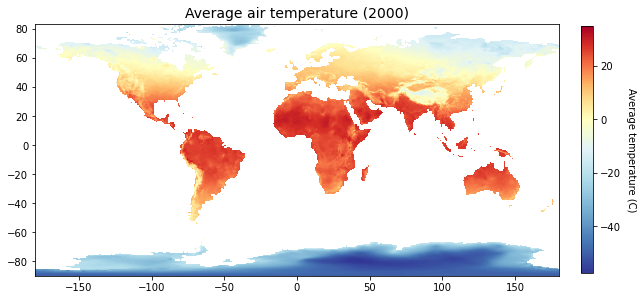
\includegraphics{./Figs/temp200.png}
\end{frame}

\begin{frame}{Krahasimi i të dhënave raster}
\protect\hypertarget{krahasimi-i-tuxeb-dhuxebnave-raster}{}
\begin{itemize}
\item
  Vizualisht, nuk është e mundur të dallohen ndryshimet midis të dhënave
  të vitit 2000 dhe atyre të vitit 2017.
\item
  Prandaj, do të zbresim dy rasterat e temperaturës, duke përdorur
  Algjebrën e Hartave.
\end{itemize}
\end{frame}

\begin{frame}{Krahasimi i të dhënave raster}
\protect\hypertarget{krahasimi-i-tuxeb-dhuxebnave-raster-1}{}
\begin{itemize}
\item
  Në praktikë, Python lejon të bëhet kjo në mënyrë intuitive si
  \textbf{raster\_vals2 - raster\_vals1}.
\item
  Këto janë operacione algjebrike lineare të aplikuara në çdo qelizë të
  matricave.
\end{itemize}
\end{frame}

\begin{frame}{Krahasimi i të dhënave raster}
\protect\hypertarget{krahasimi-i-tuxeb-dhuxebnave-raster-2}{}
\begin{itemize}
\tightlist
\item
  Pastaj do të ndërtojmë një histogram të vlerave dhe raster-it, duke
  treguar se temperaturat mesatare janë më të larta me 0.5 gradë, me
  disa raste ekstreme pozitive dhe negative që mund të shkaktohen nga
  gabimet e sensorëve.
\end{itemize}
\end{frame}

\begin{frame}{Krahasimi i të dhënave raster}
\protect\hypertarget{krahasimi-i-tuxeb-dhuxebnave-raster-3}{}
Rezultati do të ruhet në një skedar të ri raster, duke ripërdorur
metadatat nga raster-at hyrës.
\end{frame}

\begin{frame}[fragile]{Krahasimi i të dhënave raster}
\protect\hypertarget{krahasimi-i-tuxeb-dhuxebnave-raster-4}{}
\AddToHookNext{env/Highlighting/begin}{\tiny}

\begin{Shaded}
\begin{Highlighting}[]
\NormalTok{vals17 }\OperatorTok{=}\NormalTok{ temp17.read(}\DecValTok{1}\NormalTok{, masked}\OperatorTok{=}\VariableTok{True}\NormalTok{)}
\NormalTok{vals00 }\OperatorTok{=}\NormalTok{ temp00.read(}\DecValTok{1}\NormalTok{, masked}\OperatorTok{=}\VariableTok{True}\NormalTok{)}
\end{Highlighting}
\end{Shaded}
\end{frame}

\begin{frame}[fragile]{Krahasimi i të dhënave raster}
\protect\hypertarget{krahasimi-i-tuxeb-dhuxebnave-raster-5}{}
\AddToHookNext{env/Highlighting/begin}{\tiny}

\begin{Shaded}
\begin{Highlighting}[]
\CommentTok{\# zbresim të dy raster{-}at}
\NormalTok{vals\_diff }\OperatorTok{=}\NormalTok{ vals17 }\OperatorTok{{-}}\NormalTok{ vals00}
\BuiltInTok{print}\NormalTok{(}\StringTok{"Statistikat e Diferencës:"}\NormalTok{, vals\_diff.}\BuiltInTok{min}\NormalTok{(), }\BuiltInTok{round}\NormalTok{(vals\_diff.mean(), }\DecValTok{2}\NormalTok{), vals\_diff.}\BuiltInTok{max}\NormalTok{())}
\BuiltInTok{print}\NormalTok{(}\StringTok{"Diferenca midis mesatareve:"}\NormalTok{, }\BuiltInTok{round}\NormalTok{(vals17.mean()}\OperatorTok{{-}}\NormalTok{vals00.mean(), }\DecValTok{3}\NormalTok{))}
\end{Highlighting}
\end{Shaded}
\end{frame}

\begin{frame}[fragile]{Krahasimi i të dhënave raster}
\protect\hypertarget{krahasimi-i-tuxeb-dhuxebnave-raster-6}{}
\AddToHookNext{env/Highlighting/begin}{\tiny}

\begin{Shaded}
\begin{Highlighting}[]
\CommentTok{\# vizatoni histogramin}
\NormalTok{show\_hist(vals\_diff, bins}\OperatorTok{=}\DecValTok{30}\NormalTok{, lw}\OperatorTok{=}\FloatTok{0.2}\NormalTok{, stacked}\OperatorTok{=}\VariableTok{False}\NormalTok{, alpha}\OperatorTok{=}\FloatTok{0.8}\NormalTok{, label}\OperatorTok{=}\StringTok{\textquotesingle{}Nr i qelizave\textquotesingle{}}\NormalTok{,}
\NormalTok{    histtype}\OperatorTok{=}\StringTok{\textquotesingle{}stepfilled\textquotesingle{}}\NormalTok{, title}\OperatorTok{=}\StringTok{"Dallimi në temperaturën mesatare (2000{-}2017)"}\NormalTok{)}
\end{Highlighting}
\end{Shaded}
\end{frame}

\begin{frame}{Krahasimi i të dhënave raster}
\protect\hypertarget{krahasimi-i-tuxeb-dhuxebnave-raster-7}{}
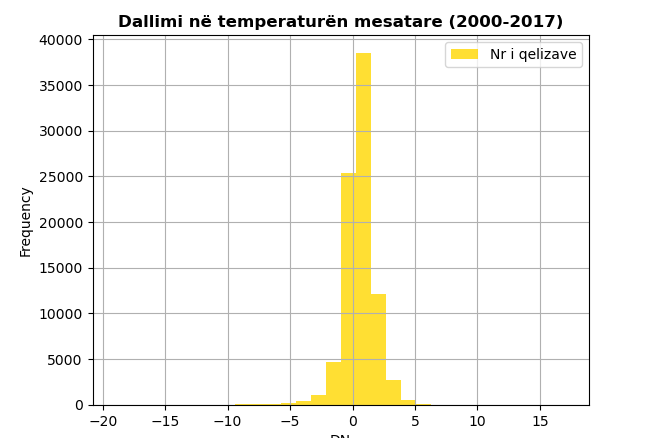
\includegraphics{./Figs/temphist.png}
\end{frame}

\begin{frame}{Ndërtojmë rasterin}
\protect\hypertarget{nduxebrtojmuxeb-rasterin}{}
\begin{itemize}
\tightlist
\item
  Cmap (Purple - White - Orange) thekson vlerat ekstreme, duke fshehur
  zonat ku vlerat nuk divergojnë.
\end{itemize}
\end{frame}

\begin{frame}[fragile]{Ndërtojmë rasterin}
\protect\hypertarget{nduxebrtojmuxeb-rasterin-1}{}
\AddToHookNext{env/Highlighting/begin}{\tiny}

\begin{Shaded}
\begin{Highlighting}[]
\NormalTok{plot\_raster(temp17, vals\_diff, }\StringTok{\textquotesingle{}Ndryshimi mesatar i temperaturës së ajrit 2000{-}2017\textquotesingle{}}\NormalTok{,}
            \StringTok{\textquotesingle{}Diferenca e temperaturës (C)\textquotesingle{}}\NormalTok{, }\StringTok{\textquotesingle{}PuOr\_r\textquotesingle{}}\NormalTok{)}
\end{Highlighting}
\end{Shaded}
\end{frame}

\begin{frame}{Ndërtojmë rasterin}
\protect\hypertarget{nduxebrtojmuxeb-rasterin-2}{}
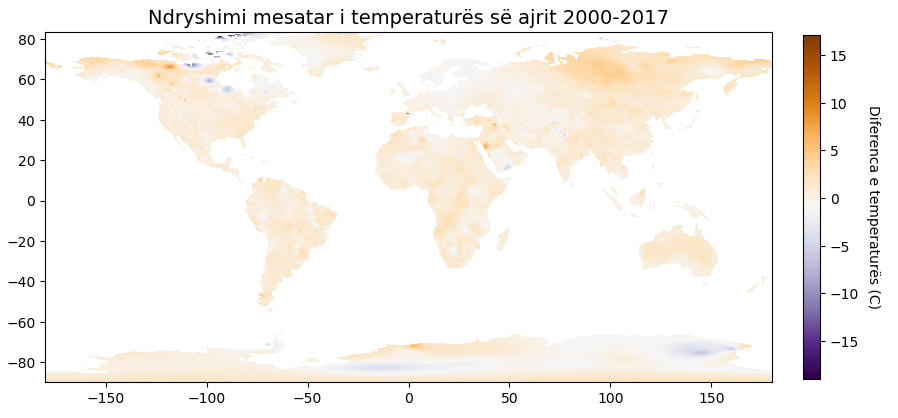
\includegraphics{./Figs/tempdif.png}
\end{frame}

\begin{frame}{Ruani rezultatin në një skedar raster}
\protect\hypertarget{ruani-rezultatin-nuxeb-njuxeb-skedar-raster}{}
\begin{itemize}
\tightlist
\item
  Është e rëndësishme të specifikohen metadatat nga skedarët hyrës,
  përfshirë CRS, vlerën NODATA dhe transformimin e koordinatave
  gjeografike:
\end{itemize}
\end{frame}

\begin{frame}[fragile]{Ruani rezultatin në një skedar raster}
\protect\hypertarget{ruani-rezultatin-nuxeb-njuxeb-skedar-raster-1}{}
\AddToHookNext{env/Highlighting/begin}{\tiny}

\begin{Shaded}
\begin{Highlighting}[]
\NormalTok{fout }\OperatorTok{=} \StringTok{\textquotesingle{}tmp/air\_temp\_diff\_2000\_2017.tif\textquotesingle{}}
\NormalTok{ds }\OperatorTok{=}\NormalTok{ rasterio.}\BuiltInTok{open}\NormalTok{(fout, }\StringTok{\textquotesingle{}w\textquotesingle{}}\NormalTok{,}
\NormalTok{    driver}\OperatorTok{=}\StringTok{\textquotesingle{}GTiff\textquotesingle{}}\NormalTok{, }\CommentTok{\# formati i skedarit të daljes}
\NormalTok{    height}\OperatorTok{=}\NormalTok{vals\_diff.shape[}\DecValTok{0}\NormalTok{], }\CommentTok{\# madhësia e matricës}
\NormalTok{    width}\OperatorTok{=}\NormalTok{vals\_diff.shape[}\DecValTok{1}\NormalTok{], }\CommentTok{\# madhësia e matricës}
\NormalTok{    count}\OperatorTok{=}\DecValTok{1}\NormalTok{, }\CommentTok{\# numri i bandave}
\NormalTok{    dtype}\OperatorTok{=}\NormalTok{vals\_diff.dtype, }\CommentTok{\# lloji i të dhënave (p.sh., pikë lundruese)}
\NormalTok{    crs}\OperatorTok{=}\NormalTok{temp17.crs, }\CommentTok{\# CRS (p.sh., Lambert, WGS84, UTM, etj.)}
\NormalTok{    nodata}\OperatorTok{=}\NormalTok{temp17.nodata, }\CommentTok{\# vlera e përdorur për të përfaqësuar NO DATA}
\NormalTok{    transform}\OperatorTok{=}\NormalTok{temp17.transform }\CommentTok{\# transformimi i koordinatave gjeografike}
\NormalTok{)}

\NormalTok{ds.write(vals\_diff, }\DecValTok{1}\NormalTok{)}
\NormalTok{ds.close()}
\BuiltInTok{print}\NormalTok{(}\StringTok{"Raster u ruajt te"}\NormalTok{, fout, }\StringTok{\textquotesingle{}.\textquotesingle{}}\NormalTok{)}
\end{Highlighting}
\end{Shaded}
\end{frame}

\begin{frame}{Statistikat zonale}
\protect\hypertarget{statistikat-zonale}{}
\begin{itemize}
\item
  Kur dëshirojmë të llogarisim statistikat raster bazuar në një zonë
  gjeografike, na duhen \textbf{statistikat zonale}.
\item
  Për shembull, mund të dëshirojmë të llogarisim lartësinë mesatare
  (vlerat) e çdo rrethi (zonave) në Angli.
\end{itemize}
\end{frame}

\begin{frame}{Statistikat zonale}
\protect\hypertarget{statistikat-zonale-1}{}
\begin{itemize}
\tightlist
\item
  Si skedar \textbf{input}, statistikat zonale kanë nevojë për një
  raster që përfaqëson vlerat dhe një grup tjetër të dhënash që
  përfaqëson zonat për të cilat duam të llogarisim statistikat:
\end{itemize}
\end{frame}

\begin{frame}{Statistikat zonale}
\protect\hypertarget{statistikat-zonale-2}{}
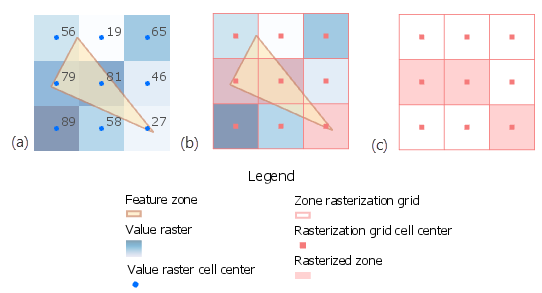
\includegraphics{./Figs/zonal1.png} \#\# Statistikat zonale

\begin{itemize}
\tightlist
\item
  Në këtë shembull, ne do të përdorim të dhënat evropiane të NOx të
  përdorura më sipër si vlera dhe zonat statistikore evropiane (NUTS) si
  zona.
\end{itemize}
\end{frame}

\begin{frame}[fragile]{Shkarkojmë datat}
\protect\hypertarget{shkarkojmuxeb-datat}{}
\AddToHookNext{env/Highlighting/begin}{\tiny}

\begin{Shaded}
\begin{Highlighting}[]
\CommentTok{\# shkarkoni kufijtë rajonalë të BE{-}së (niveli NUTS 2, 2021)}
\NormalTok{nuts2\_file }\OperatorTok{=} \StringTok{\textquotesingle{}data/NUTS\_RG\_01M\_2021\_4326\_LEVL\_2.geojson.gz\textquotesingle{}}
\NormalTok{url }\OperatorTok{=} \StringTok{\textquotesingle{}https://raw.githubusercontent.com/endri81/instatgis/master/data/gis4/NUTS\_RG\_01M\_2021\_4326\_LEVL\_2.geojson.gz\textquotesingle{}}
\NormalTok{urllib.request.urlretrieve(url, nuts2\_file)}
\end{Highlighting}
\end{Shaded}
\end{frame}

\begin{frame}[fragile]{Shkarkojmë datat}
\protect\hypertarget{shkarkojmuxeb-datat-1}{}
Skedari është gzip dhe mund ta hapim direkt me
\textbf{gzip.open(\ldots)}

\AddToHookNext{env/Highlighting/begin}{\tiny}

\begin{Shaded}
\begin{Highlighting}[]
\ImportTok{import}\NormalTok{ geopandas }\ImportTok{as}\NormalTok{ gpd}
\ImportTok{import}\NormalTok{ gzip}
\NormalTok{nuts2\_df }\OperatorTok{=}\NormalTok{ gpd.read\_file(gzip.}\BuiltInTok{open}\NormalTok{(nuts2\_file))}
\NormalTok{nuts2\_df.plot()}
\end{Highlighting}
\end{Shaded}
\end{frame}

\begin{frame}{Shkarkojmë datat}
\protect\hypertarget{shkarkojmuxeb-datat-2}{}
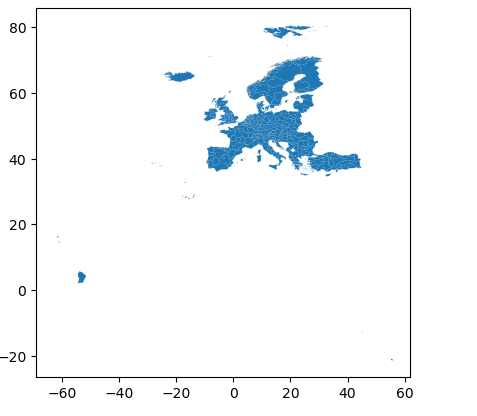
\includegraphics{./Figs/gzip.png}
\end{frame}

\begin{frame}[fragile]{Kontrollojmë}
\protect\hypertarget{kontrollojmuxeb}{}
\AddToHookNext{env/Highlighting/begin}{\tiny}

\begin{Shaded}
\begin{Highlighting}[]
\NormalTok{nuts2\_df.sample(}\DecValTok{5}\NormalTok{)}
\end{Highlighting}
\end{Shaded}
\end{frame}

\begin{frame}{Përgatitja e të Dhënave}
\protect\hypertarget{puxebrgatitja-e-tuxeb-dhuxebnave}{}
\begin{itemize}
\tightlist
\item
  Duke qenë se nuk kemi të dhëna për Guyana Franceze dhe territore të
  tjera më të vogla, mund t'i heqim ato nga dataset-i.
\end{itemize}
\end{frame}

\begin{frame}[fragile]{Përgatitja e të Dhënave}
\protect\hypertarget{puxebrgatitja-e-tuxeb-dhuxebnave-1}{}
Në dataframe pandas, mund të shkruajmë kushte në mënyra të ndryshme:

\begin{itemize}
\item
  \texttt{column.str.contains(string)} kryen një përputhje të pjesshme
  në një kolonë me format tekst
\item
  \texttt{column.isin(list)} kryen një përputhje të saktë në përmbajtjen
  e një kolone ndaj një liste
\item
  \texttt{\textasciitilde{}} do të thotë ``jo'' (vetëm në kontekstin e
  pandas)
\end{itemize}
\end{frame}

\begin{frame}{Përgatitja e të Dhënave}
\protect\hypertarget{puxebrgatitja-e-tuxeb-dhuxebnave-2}{}
\begin{itemize}
\item
  Do projektojmë kufijtë dhe ti ruajmë ato në një GeoPackage.
\item
  Kini parasysh se GeoJSON lejon vetëm gjeometri në WGS84 (4326).
\item
  Kur keni një CRS tjetër, duhet të përdorni një GeoPackage.
\end{itemize}
\end{frame}

\begin{frame}[fragile]{Përgatitja e të Dhënave}
\protect\hypertarget{puxebrgatitja-e-tuxeb-dhuxebnave-3}{}
\AddToHookNext{env/Highlighting/begin}{\tiny}

\begin{Shaded}
\begin{Highlighting}[]
\CommentTok{\# Kjo shprehje do të thotë:}
\CommentTok{\# zgjidhni rreshta ku NUTS\_ID nuk përmban \textquotesingle{}FRY\textquotesingle{}}
\NormalTok{nuts2\_df }\OperatorTok{=}\NormalTok{ nuts2\_df[}\OperatorTok{\textasciitilde{}}\NormalTok{nuts2\_df[}\StringTok{\textquotesingle{}NUTS\_ID\textquotesingle{}}\NormalTok{].}\BuiltInTok{str}\NormalTok{.contains(}\StringTok{"FRY"}\NormalTok{)]}

\CommentTok{\# hiqni rreshtat me kode që korrespondojnë me ishujt për të cilët nuk kemi të dhëna:}
\NormalTok{nuts2\_df }\OperatorTok{=}\NormalTok{ nuts2\_df[}\OperatorTok{\textasciitilde{}}\NormalTok{nuts2\_df[}\StringTok{\textquotesingle{}NUTS\_ID\textquotesingle{}}\NormalTok{].isin([}\StringTok{\textquotesingle{}PT20\textquotesingle{}}\NormalTok{,}\StringTok{\textquotesingle{}PT30\textquotesingle{}}\NormalTok{,}\StringTok{\textquotesingle{}ES70\textquotesingle{}}\NormalTok{,}\StringTok{\textquotesingle{}NO0B\textquotesingle{}}\NormalTok{])]}

\CommentTok{\# projektoni në Lambert (i përshtatshëm për Evropën)}
\NormalTok{nuts2\_df }\OperatorTok{=}\NormalTok{ nuts2\_df.to\_crs(}\DecValTok{3035}\NormalTok{)}
\NormalTok{nuts2\_df.info()}

\CommentTok{\# Ky është një rregullim: dataframe gjeo kanë nevojë që FID të jetë i tipit integer}
\NormalTok{nuts2\_df[}\StringTok{\textquotesingle{}FID\textquotesingle{}}\NormalTok{] }\OperatorTok{=}\NormalTok{ nuts2\_df.index}
\end{Highlighting}
\end{Shaded}
\end{frame}

\begin{frame}[fragile]{Ruani këtë dataset në një skedar}
\protect\hypertarget{ruani-kuxebtuxeb-dataset-nuxeb-njuxeb-skedar}{}
\AddToHookNext{env/Highlighting/begin}{\tiny}

\begin{Shaded}
\begin{Highlighting}[]
\NormalTok{nuts2\_clean\_file }\OperatorTok{=} \StringTok{"tmp/nuts2\_boundaries.gpkg"}
\NormalTok{nuts2\_df.to\_file(nuts2\_clean\_file, driver}\OperatorTok{=}\StringTok{"GPKG"}\NormalTok{)}
\end{Highlighting}
\end{Shaded}
\end{frame}

\begin{frame}[fragile]{Vizatoni gjeometrinë}
\protect\hypertarget{vizatoni-gjeometrinuxeb}{}
\AddToHookNext{env/Highlighting/begin}{\tiny}

\begin{Shaded}
\begin{Highlighting}[]
\NormalTok{nuts2\_df.plot(figsize}\OperatorTok{=}\NormalTok{(}\DecValTok{10}\NormalTok{,}\DecValTok{10}\NormalTok{))}
\end{Highlighting}
\end{Shaded}
\end{frame}

\begin{frame}{Vizatoni gjeometrinë}
\protect\hypertarget{vizatoni-gjeometrinuxeb-1}{}
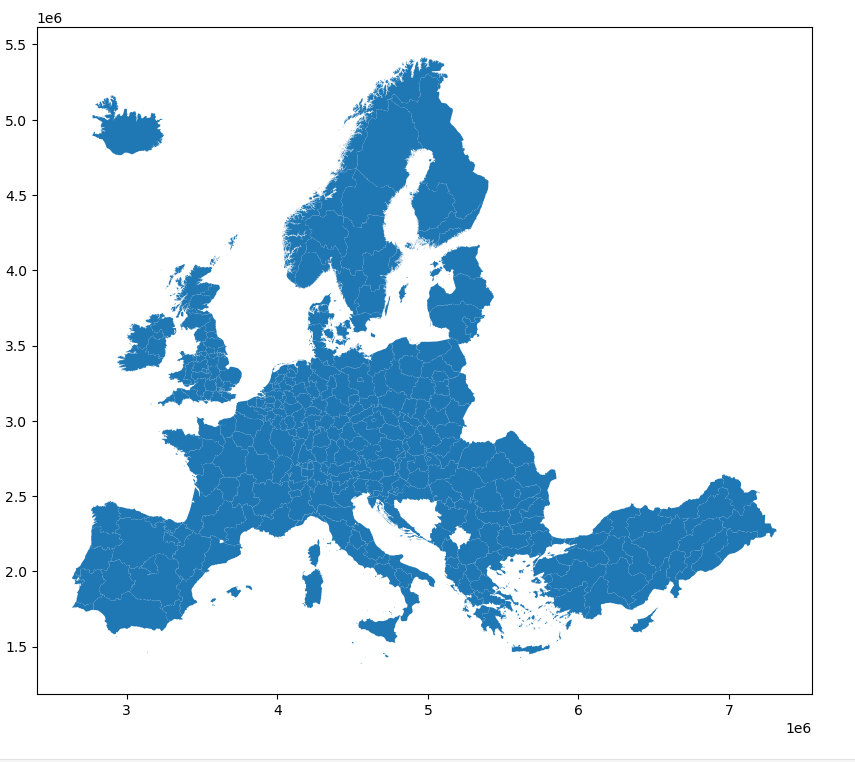
\includegraphics{./Figs/algebra1.png}
\end{frame}

\begin{frame}[fragile]{Statistikat Zonale në Python}
\protect\hypertarget{statistikat-zonale-nuxeb-python}{}
\begin{itemize}
\item
  Statistikat zonale mund të llogariten me funksionin
  \textbf{rasterstats.zonal\_stats}
\item
  Parametri \texttt{stats} tregon cilat statistika dëshirojmë të
  llogariten në çdo zonë.
\end{itemize}
\end{frame}

\begin{frame}{Statistikat Zonale në Python}
\protect\hypertarget{statistikat-zonale-nuxeb-python-1}{}
\begin{itemize}
\tightlist
\item
  Do të llogarisim disa statistika zonale dhe do ta ruajmë rezultatin në
  një GeoPackage dhe një skedar CSV:
\end{itemize}
\end{frame}

\begin{frame}[fragile]{Statistikat Zonale në Python}
\protect\hypertarget{statistikat-zonale-nuxeb-python-2}{}
\AddToHookNext{env/Highlighting/begin}{\tiny}

\begin{Shaded}
\begin{Highlighting}[]
\ImportTok{from}\NormalTok{ rasterstats }\ImportTok{import}\NormalTok{ zonal\_stats}

\BuiltInTok{print}\NormalTok{(}\StringTok{"Duke llogaritur statistikat zonale midis"}\NormalTok{, nuts2\_clean\_file, }\StringTok{\textquotesingle{}dhe data/eu{-}2016{-}nox\_avg.tif ...\textquotesingle{}}\NormalTok{)}

\NormalTok{zon\_stats }\OperatorTok{=}\NormalTok{ zonal\_stats(nuts2\_clean\_file, }\StringTok{\textquotesingle{}data/eu{-}2016{-}nox\_avg.tif\textquotesingle{}}\NormalTok{,}
\NormalTok{                        stats}\OperatorTok{=}\StringTok{"count min mean max median"}\NormalTok{, geojson\_out}\OperatorTok{=}\VariableTok{True}\NormalTok{)}
\BuiltInTok{print}\NormalTok{(}\StringTok{\textquotesingle{}Përfunduar.\textquotesingle{}}\NormalTok{)}
\end{Highlighting}
\end{Shaded}
\end{frame}

\begin{frame}{Statistikat Zonale në Python}
\protect\hypertarget{statistikat-zonale-nuxeb-python-3}{}
\begin{itemize}
\item
  Rezultati është një listë e fjalorëve që përmban statistikat për çdo
  rresht të skedarit hyrës të vektorit
\item
  Këto rezultate mund të konvertohen në një kornizë të të dhënave gjeo
  kështu:
\end{itemize}
\end{frame}

\begin{frame}[fragile]{Statistikat Zonale në Python}
\protect\hypertarget{statistikat-zonale-nuxeb-python-4}{}
\AddToHookNext{env/Highlighting/begin}{\tiny}

\begin{Shaded}
\begin{Highlighting}[]
\ImportTok{import}\NormalTok{ geopandas }\ImportTok{as}\NormalTok{ gpd}
\NormalTok{stats\_df }\OperatorTok{=}\NormalTok{ gpd.GeoDataFrame.from\_features(zon\_stats)}

\CommentTok{\# riemërtoni kolonat për të qenë më kuptimplota}
\NormalTok{stats\_df }\OperatorTok{=}\NormalTok{ stats\_df.rename(columns}\OperatorTok{=}\NormalTok{\{}\StringTok{"min"}\NormalTok{: }\StringTok{"nox\_min"}\NormalTok{,}
                                    \StringTok{"max"}\NormalTok{: }\StringTok{"nox\_max"}\NormalTok{,}
                                    \StringTok{"count"}\NormalTok{: }\StringTok{"nox\_count"}\NormalTok{,}
                                    \StringTok{"mean"}\NormalTok{: }\StringTok{"nox\_mean"}\NormalTok{,}
                                    \StringTok{"median"}\NormalTok{: }\StringTok{"nox\_median"}\NormalTok{\})}
\NormalTok{stats\_df.sample(}\DecValTok{4}\NormalTok{)}
\end{Highlighting}
\end{Shaded}
\end{frame}

\begin{frame}{Statistikat Zonale në Python}
\protect\hypertarget{statistikat-zonale-nuxeb-python-5}{}
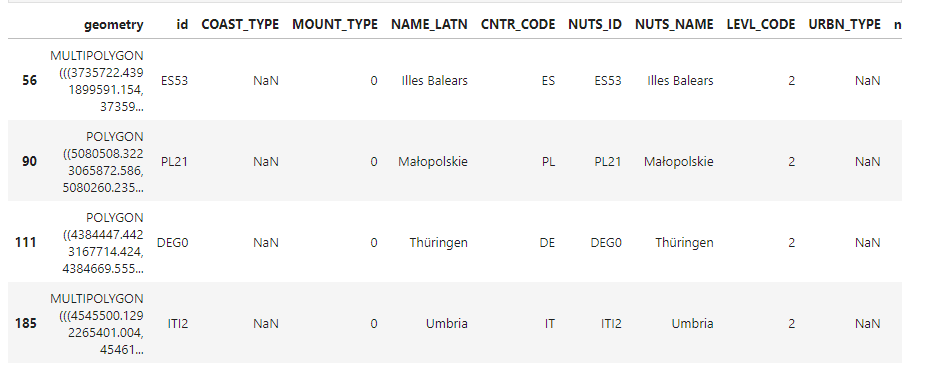
\includegraphics{./Figs/regstat.png}
\end{frame}

\begin{frame}[fragile]{Statistikat Zonale në Python}
\protect\hypertarget{statistikat-zonale-nuxeb-python-6}{}
\AddToHookNext{env/Highlighting/begin}{\tiny}

\begin{Shaded}
\begin{Highlighting}[]
\CommentTok{\# ruajmë rezultatin në një geopackage}
\NormalTok{stats\_df.to\_file(}\StringTok{\textquotesingle{}tmp/eu\_nox\_2016\_nuts2.gpkg\textquotesingle{}}\NormalTok{, driver}\OperatorTok{=}\StringTok{"GPKG"}\NormalTok{)}

\CommentTok{\# për lehtësi ruajmë tabelën e atributeve si CSV}
\NormalTok{stats\_df.drop(columns}\OperatorTok{=}\NormalTok{[}\StringTok{\textquotesingle{}geometry\textquotesingle{}}\NormalTok{]).to\_csv(}\StringTok{\textquotesingle{}tmp/eu\_nox\_2016\_nuts2.csv\textquotesingle{}}\NormalTok{, index}\OperatorTok{=}\VariableTok{False}\NormalTok{)}
\BuiltInTok{print}\NormalTok{(}\StringTok{"results saved."}\NormalTok{)}
\end{Highlighting}
\end{Shaded}
\end{frame}

\begin{frame}{Renditja dhe Vizualizimi i Rezultateve}
\protect\hypertarget{renditja-dhe-vizualizimi-i-rezultateve}{}
\begin{itemize}
\item
  Tani, ne mund të eksplorojmë dhe vizualizojmë rezultatet.
\item
  Funksioni \textbf{.rank()} i pandas na lejon të renditim vlerat.
\end{itemize}
\end{frame}

\begin{frame}{Renditja dhe Vizualizimi i Rezultateve}
\protect\hypertarget{renditja-dhe-vizualizimi-i-rezultateve-1}{}
\begin{itemize}
\item
  Shpesh është një ide e mirë të ndajmë në qeliza të ndryshme
  llogaritjet dhe vizualizimet e gjata.
\item
  Në këtë rast, nëse dëshirojmë të ekzekutojmë vizualizime të ndryshme,
  nuk kemi nevojë të rikthejmë llogaritjet zonale në qelizën e
  mëparshme.
\end{itemize}
\end{frame}

\begin{frame}[fragile]{Renditja dhe Vizualizimi i Rezultateve}
\protect\hypertarget{renditja-dhe-vizualizimi-i-rezultateve-2}{}
\AddToHookNext{env/Highlighting/begin}{\tiny}

\begin{Shaded}
\begin{Highlighting}[]
\NormalTok{nox\_nuts2\_df }\OperatorTok{=}\NormalTok{ gpd.read\_file(}\StringTok{\textquotesingle{}tmp/eu\_nox\_2016\_nuts2.gpkg\textquotesingle{}}\NormalTok{)}
\BuiltInTok{print}\NormalTok{(nox\_nuts2\_df.describe())}
\BuiltInTok{print}\NormalTok{(nox\_nuts2\_df.columns)}
\end{Highlighting}
\end{Shaded}
\end{frame}

\begin{frame}{Renditja dhe Vizualizimi i Rezultateve}
\protect\hypertarget{renditja-dhe-vizualizimi-i-rezultateve-3}{}
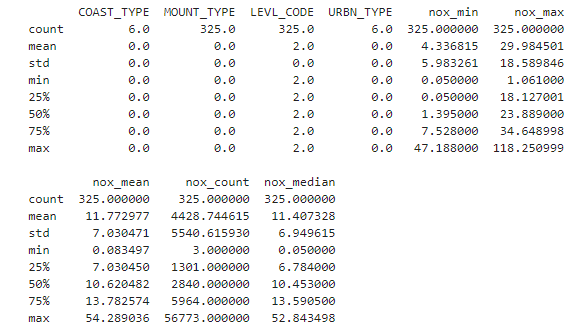
\includegraphics{./Figs/eunox.png}
\end{frame}

\begin{frame}[fragile]{Renditja dhe Vizualizimi i Rezultateve}
\protect\hypertarget{renditja-dhe-vizualizimi-i-rezultateve-4}{}
\AddToHookNext{env/Highlighting/begin}{\tiny}

\begin{Shaded}
\begin{Highlighting}[]
\CommentTok{\# Rendisni rajonet: 1 = vlera më e lartë}
\NormalTok{nox\_nuts2\_df[}\StringTok{\textquotesingle{}nox\_mean\_rank\textquotesingle{}}\NormalTok{] }\OperatorTok{=}\NormalTok{ nox\_nuts2\_df[}\StringTok{\textquotesingle{}nox\_mean\textquotesingle{}}\NormalTok{].rank(ascending}\OperatorTok{=}\VariableTok{False}\NormalTok{)}
\NormalTok{nox\_nuts2\_df[}\StringTok{\textquotesingle{}nox\_max\_rank\textquotesingle{}}\NormalTok{] }\OperatorTok{=}\NormalTok{ nox\_nuts2\_df[}\StringTok{\textquotesingle{}nox\_max\textquotesingle{}}\NormalTok{].rank(ascending}\OperatorTok{=}\VariableTok{False}\NormalTok{)}
\end{Highlighting}
\end{Shaded}
\end{frame}

\begin{frame}[fragile]{Renditja dhe Vizualizimi i Rezultateve}
\protect\hypertarget{renditja-dhe-vizualizimi-i-rezultateve-5}{}
\AddToHookNext{env/Highlighting/begin}{\tiny}

\begin{Shaded}
\begin{Highlighting}[]
\CommentTok{\# E vërtetë nëse vlera \textgreater{} 40}
\NormalTok{nox\_nuts2\_df[}\StringTok{\textquotesingle{}nox\_max\_high\textquotesingle{}}\NormalTok{] }\OperatorTok{=}\NormalTok{ nox\_nuts2\_df[}\StringTok{\textquotesingle{}nox\_max\textquotesingle{}}\NormalTok{] }\OperatorTok{\textgreater{}} \DecValTok{40}
\end{Highlighting}
\end{Shaded}
\end{frame}

\begin{frame}[fragile]{Renditja dhe Vizualizimi i Rezultateve}
\protect\hypertarget{renditja-dhe-vizualizimi-i-rezultateve-6}{}
\AddToHookNext{env/Highlighting/begin}{\tiny}

\begin{Shaded}
\begin{Highlighting}[]
\CommentTok{\# Shikoni rajonet më të ndotura NUTS, duke përzgjedhur vetëm kolonat përkatëse}
\NormalTok{sel\_df }\OperatorTok{=}\NormalTok{ nox\_nuts2\_df[[}\StringTok{\textquotesingle{}NUTS\_ID\textquotesingle{}}\NormalTok{,}\StringTok{\textquotesingle{}NUTS\_NAME\textquotesingle{}}\NormalTok{,}\StringTok{\textquotesingle{}nox\_mean\textquotesingle{}}\NormalTok{,}\StringTok{\textquotesingle{}nox\_max\textquotesingle{}}\NormalTok{,}
                       \StringTok{\textquotesingle{}nox\_mean\_rank\textquotesingle{}}\NormalTok{,}\StringTok{\textquotesingle{}nox\_max\_rank\textquotesingle{}}\NormalTok{,}\StringTok{\textquotesingle{}nox\_max\_high\textquotesingle{}}\NormalTok{]]}
\NormalTok{sel\_df.sample(}\DecValTok{5}\NormalTok{)}

\CommentTok{\# Rendisni rajonet sipas nox\_mean}
\NormalTok{sel\_df.sort\_values(}\StringTok{\textquotesingle{}nox\_mean\textquotesingle{}}\NormalTok{,ascending}\OperatorTok{=}\VariableTok{False}\NormalTok{).head(}\DecValTok{20}\NormalTok{)}
\end{Highlighting}
\end{Shaded}
\end{frame}

\begin{frame}{Renditja dhe Vizualizimi i Rezultateve}
\protect\hypertarget{renditja-dhe-vizualizimi-i-rezultateve-7}{}
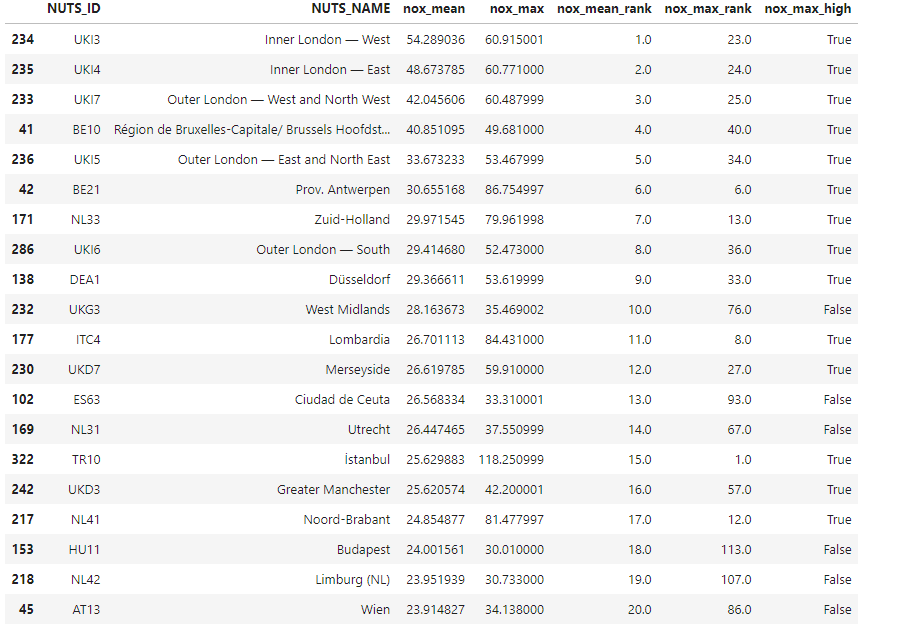
\includegraphics{./Figs/eunox2.png}
\end{frame}

\begin{frame}{Renditja dhe Vizualizimi i Rezultateve}
\protect\hypertarget{renditja-dhe-vizualizimi-i-rezultateve-8}{}
\begin{itemize}
\item
  Vini re se si renditja për \textbf{nox\_max} dhe \textbf{nox\_mean}
  mund të ndryshojë:
\item
  Për shembull, Inner London - West (``UKI3'') ka nivelin më të lartë të
  NOx në mesatare, por është vetëm i 23-ti për sa i përket vlerës
  maksimale.
\end{itemize}
\end{frame}

\begin{frame}[fragile]{Renditja dhe Vizualizimi i Rezultateve}
\protect\hypertarget{renditja-dhe-vizualizimi-i-rezultateve-9}{}
\begin{itemize}
\tightlist
\item
  Mund të vizatojmë vlerat e grumbulluara me një choropleth:
\end{itemize}

\AddToHookNext{env/Highlighting/begin}{\tiny}

\begin{Shaded}
\begin{Highlighting}[]
\NormalTok{nox\_nuts2\_df.plot(column}\OperatorTok{=}\StringTok{\textquotesingle{}nox\_max\textquotesingle{}}\NormalTok{, figsize}\OperatorTok{=}\NormalTok{(}\DecValTok{12}\NormalTok{,}\DecValTok{9}\NormalTok{), scheme}\OperatorTok{=}\StringTok{\textquotesingle{}equalinterval\textquotesingle{}}\NormalTok{, cmap}\OperatorTok{=}\StringTok{\textquotesingle{}OrRd\textquotesingle{}}\NormalTok{, k}\OperatorTok{=}\DecValTok{5}\NormalTok{,}
\NormalTok{    edgecolor}\OperatorTok{=}\StringTok{"lightgrey"}\NormalTok{, linewidth}\OperatorTok{=}\FloatTok{0.4}\NormalTok{,}
\NormalTok{    legend}\OperatorTok{=}\VariableTok{True}\NormalTok{, legend\_kwds}\OperatorTok{=}\NormalTok{\{}\StringTok{\textquotesingle{}loc\textquotesingle{}}\NormalTok{: }\StringTok{\textquotesingle{}upper right\textquotesingle{}}\NormalTok{, }\StringTok{\textquotesingle{}title\textquotesingle{}}\NormalTok{: }\StringTok{\textquotesingle{}NOx Maksimale (2016) {-} NUTS 2\textquotesingle{}}\NormalTok{\},}
\NormalTok{    missing\_kwds}\OperatorTok{=}\NormalTok{\{}\StringTok{\textquotesingle{}color\textquotesingle{}}\NormalTok{: }\StringTok{"lightgrey"}\NormalTok{\})}
\end{Highlighting}
\end{Shaded}
\end{frame}

\begin{frame}{Renditja dhe Vizualizimi i Rezultateve}
\protect\hypertarget{renditja-dhe-vizualizimi-i-rezultateve-10}{}
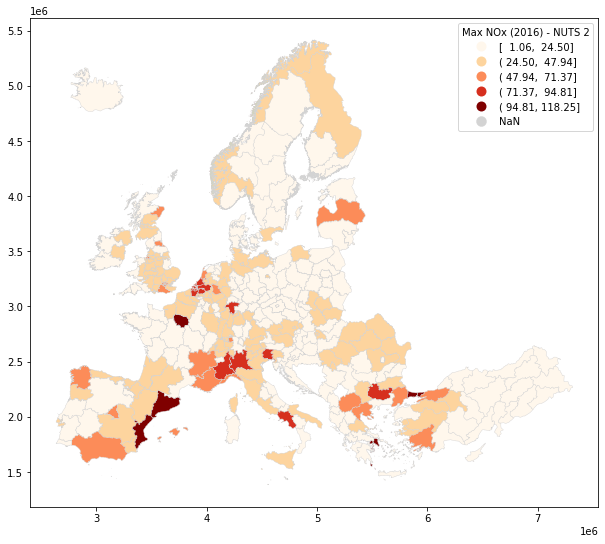
\includegraphics{./Figs/eunox3.png}
\end{frame}

\begin{frame}{Renditja dhe Vizualizimi i Rezultateve}
\protect\hypertarget{renditja-dhe-vizualizimi-i-rezultateve-11}{}
\begin{itemize}
\item
  Shpërndarja e NOx është shumë heterogjene hapësinore (dmth., ndryshon
  shumë në çdo vend).
\item
  Ne mund të përdorim \textbf{groupby} për të gjetur njësinë kryesore të
  NUTS për çdo vend për sa i përket NOx maksimale:
\end{itemize}
\end{frame}

\begin{frame}[fragile]{Renditja dhe Vizualizimi i Rezultateve}
\protect\hypertarget{renditja-dhe-vizualizimi-i-rezultateve-12}{}
\AddToHookNext{env/Highlighting/begin}{\tiny}

\begin{Shaded}
\begin{Highlighting}[]
\NormalTok{nox\_nuts2\_df[}\StringTok{\textquotesingle{}nox\_max\_country\_rank\textquotesingle{}}\NormalTok{] }\OperatorTok{=}\NormalTok{ nox\_nuts2\_df.groupby(}\StringTok{\textquotesingle{}CNTR\_CODE\textquotesingle{}}\NormalTok{)[}\StringTok{\textquotesingle{}nox\_max\textquotesingle{}}\NormalTok{].rank(ascending}\OperatorTok{=}\VariableTok{False}\NormalTok{)}

\CommentTok{\# për çdo vend, njësitë renditen në mënyrë të brendshme}
\NormalTok{sel\_df }\OperatorTok{=}\NormalTok{ nox\_nuts2\_df[[}\StringTok{\textquotesingle{}NUTS\_ID\textquotesingle{}}\NormalTok{,}\StringTok{\textquotesingle{}NUTS\_NAME\textquotesingle{}}\NormalTok{,}\StringTok{\textquotesingle{}nox\_max\textquotesingle{}}\NormalTok{,}\StringTok{\textquotesingle{}nox\_max\_country\_rank\textquotesingle{}}\NormalTok{]]}
\NormalTok{sel\_df}
\end{Highlighting}
\end{Shaded}
\end{frame}

\begin{frame}[fragile]{Renditja dhe Vizualizimi i Rezultateve}
\protect\hypertarget{renditja-dhe-vizualizimi-i-rezultateve-13}{}
\AddToHookNext{env/Highlighting/begin}{\tiny}

\begin{Shaded}
\begin{Highlighting}[]
\CommentTok{\# Zgjidhni vetëm njësinë kryesore për çdo vend (rank==1) dhe rendisni ato sipas NOx maksimale:}
\NormalTok{top\_df }\OperatorTok{=}\NormalTok{ sel\_df[sel\_df[}\StringTok{\textquotesingle{}nox\_max\_country\_rank\textquotesingle{}}\NormalTok{]}\OperatorTok{==}\DecValTok{1}\NormalTok{]}
\NormalTok{top\_df.sort\_values(}\StringTok{\textquotesingle{}nox\_max\textquotesingle{}}\NormalTok{, ascending}\OperatorTok{=}\VariableTok{False}\NormalTok{)}
\end{Highlighting}
\end{Shaded}
\end{frame}

\begin{frame}{Renditja dhe Vizualizimi i Rezultateve}
\protect\hypertarget{renditja-dhe-vizualizimi-i-rezultateve-14}{}
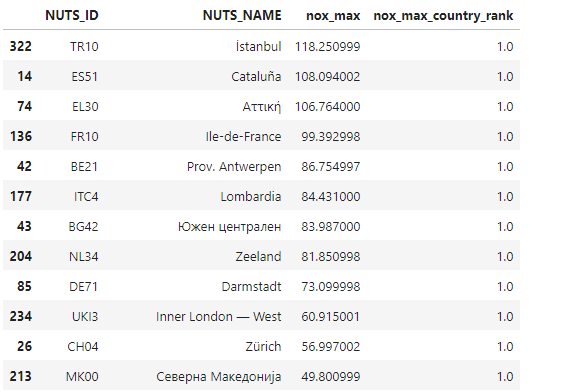
\includegraphics{./Figs/eunox4.png}
\end{frame}

\hypertarget{praktikuxeb}{%
\section{Praktikë}\label{praktikuxeb}}

\begin{frame}{Detyra 1}
\protect\hypertarget{detyra-1}{}
\begin{itemize}
\item
  Do ngarkojmë dataset që përmban raster me të dhëna globale të reshjeve
  nga viti 1950 deri në vitin 2017 në milimetra nga url
  \href{https://raw.githubusercontent.com/endri81/instatgis/master/data/global_precipitation_1950_2017/rasters/}{https://raw.githubusercontent.com/endri81/instatgis/master/data/global\_precipitation\_1950\_2017/
  rasters/}
\item
  Duke përdorur cikle for, merrni raster-in e reshjeve çdo 5 vjet nga
  viti 1980 deri në vitin 2015.
\item
  Për çdo raster, gjeneroni një grafik duke përdorur funksionin
  \textbf{plot\_raster} (funksioni në 2 slidet e tjera) dhe printoni
  vlerat minimale, mesatare dhe maksimale.
\end{itemize}
\end{frame}

\begin{frame}[fragile]{Funksioni plot\_raster}
\protect\hypertarget{funksioni-plot_raster}{}
\AddToHookNext{env/Highlighting/begin}{\tiny}

\begin{Shaded}
\begin{Highlighting}[]
\CommentTok{\# Duke qenë se funksionaliteti i vizualizimit të rasterio është mjaft i komplikuar,}
\CommentTok{\# ne krijojmë një funksion për të vizualizuar një raster më lehtë.}
\CommentTok{\# Vini re vlerat e paracaktuara (Blues, 10, 10).}
\CommentTok{\# Sa i përket kompleksitetit, kjo është një funksion realist i përdorur në shkencën e të dhënave,}
\CommentTok{\# me "hack"{-}e për t\textquotesingle{}i bërë gjërat të funksionojnë për shkak të kufizimeve të paketës.}

\KeywordTok{def}\NormalTok{ plot\_raster(rast, val\_matrix, plot\_title, value\_label, cmap}\OperatorTok{=}\StringTok{\textquotesingle{}Blues\textquotesingle{}}\NormalTok{, width}\OperatorTok{=}\DecValTok{10}\NormalTok{, height}\OperatorTok{=}\DecValTok{10}\NormalTok{, diverge\_zero}\OperatorTok{=}\VariableTok{False}\NormalTok{):}
    \CommentTok{"""Vizualizon një rasterio raster me cilësime të arsyeshme dhe me legjendë.}
\CommentTok{        @ rast: skedari rasterio (përdoret për të lexuar koordinatat gjeografike)}
\CommentTok{        @ val\_matrix: vlerat e nxjerra (përdoret për të lexuar vlerat e rasterit)}
\CommentTok{        @ plot\_title: titulli i figurës së plotë}
\CommentTok{        @ value\_label: sasia që shfaqet}
\CommentTok{        @ diverge\_zero: e vërtetë nëse përdorni një cmap divergjent për të përqendruar hartën e ngjyrave në zero}
\CommentTok{    """}
\NormalTok{    fig, ax }\OperatorTok{=}\NormalTok{ plt.subplots(figsize}\OperatorTok{=}\NormalTok{(}\DecValTok{10}\NormalTok{,}\DecValTok{10}\NormalTok{))}
    \CommentTok{\# image\_hidden është një "hack" për të treguar legjendën}
    \ControlFlowTok{if}\NormalTok{ diverge\_zero:}
\NormalTok{        image\_hidden }\OperatorTok{=}\NormalTok{ ax.imshow(val\_matrix, cmap}\OperatorTok{=}\NormalTok{cmap, norm}\OperatorTok{=}\NormalTok{TwoSlopeNorm(}\DecValTok{0}\NormalTok{))}
    \ControlFlowTok{else}\NormalTok{:}
\NormalTok{        image\_hidden }\OperatorTok{=}\NormalTok{ ax.imshow(val\_matrix, cmap}\OperatorTok{=}\NormalTok{cmap)}

\NormalTok{    ax.clear()}
\end{Highlighting}
\end{Shaded}
\end{frame}

\begin{frame}[fragile]{Funksioni plot\_raster (vazhdim)}
\protect\hypertarget{funksioni-plot_raster-vazhdim}{}
\AddToHookNext{env/Highlighting/begin}{\tiny}

\begin{Shaded}
\begin{Highlighting}[]
    \CommentTok{\# vizualizoni raster: rast.transform lejon sistemin të tregojë koordinatat gjeografike}
    \ControlFlowTok{if}\NormalTok{ diverge\_zero:}
\NormalTok{        rast\_plot }\OperatorTok{=}\NormalTok{ rasterio.plot.show(val\_matrix, cmap}\OperatorTok{=}\NormalTok{cmap, ax}\OperatorTok{=}\NormalTok{ax, transform}\OperatorTok{=}\NormalTok{rast.transform, norm}\OperatorTok{=}\NormalTok{TwoSlopeNorm(}\DecValTok{0}\NormalTok{))}
    \ControlFlowTok{else}\NormalTok{: }
\NormalTok{        rast\_plot }\OperatorTok{=}\NormalTok{ rasterio.plot.show(val\_matrix, cmap}\OperatorTok{=}\NormalTok{cmap, ax}\OperatorTok{=}\NormalTok{ax, transform}\OperatorTok{=}\NormalTok{rast.transform)}
    
    \CommentTok{\# vendosni titullin e grafikut}
\NormalTok{    ax.set\_title(plot\_title, fontsize}\OperatorTok{=}\DecValTok{14}\NormalTok{)}
    
    \CommentTok{\# shfaqni legjendën me etiketën}
    \CommentTok{\# "hack" për të rregulluar lartësinë}
\NormalTok{    im\_ratio }\OperatorTok{=}\NormalTok{ val\_matrix.shape[}\DecValTok{0}\NormalTok{]}\OperatorTok{/}\NormalTok{val\_matrix.shape[}\DecValTok{1}\NormalTok{] }
    \CommentTok{\#plt.colorbar(im,fraction=0.046*im\_ratio, pad=0.04)}
\NormalTok{    cbar }\OperatorTok{=}\NormalTok{ fig.colorbar(image\_hidden, ax}\OperatorTok{=}\NormalTok{ax, fraction}\OperatorTok{=}\FloatTok{0.046}\OperatorTok{*}\NormalTok{im\_ratio, pad}\OperatorTok{=}\FloatTok{0.04}\NormalTok{)}
\NormalTok{    cbar.ax.set\_ylabel(value\_label, rotation}\OperatorTok{=}\DecValTok{270}\NormalTok{)}
\NormalTok{    cbar.ax.get\_yaxis().labelpad }\OperatorTok{=} \DecValTok{15}
    \CommentTok{\#ax.set\_axis\_off() \# aktivizoni/çaktivizoni akset}
\NormalTok{    plt.show()}
\end{Highlighting}
\end{Shaded}
\end{frame}

\begin{frame}[fragile]{Zgjidhje}
\protect\hypertarget{zgjidhje}{}
\AddToHookNext{env/Highlighting/begin}{\tiny}

\begin{Shaded}
\begin{Highlighting}[]
\ImportTok{import}\NormalTok{ urllib.request}

\CommentTok{\# shkarkoni skedarët. Asc qëndron për Ascii, një format i thjeshtë raster.}
\NormalTok{years }\OperatorTok{=} \BuiltInTok{range}\NormalTok{(}\DecValTok{1980}\NormalTok{, }\DecValTok{2016}\NormalTok{, }\DecValTok{5}\NormalTok{)}
\NormalTok{base\_url }\OperatorTok{=} \StringTok{\textquotesingle{}https://raw.githubusercontent.com/endri81/instatgis/master/data/global\_precipitation\_1950\_2017/rasters/\textquotesingle{}}

\ControlFlowTok{for}\NormalTok{ year }\KeywordTok{in}\NormalTok{ years:}
\NormalTok{    rast\_url }\OperatorTok{=}\NormalTok{ base\_url }\OperatorTok{+} \StringTok{\textquotesingle{}precip\_}\SpecialCharTok{\{\}}\StringTok{{-}total.asc\textquotesingle{}}\NormalTok{.}\BuiltInTok{format}\NormalTok{(year)}
\NormalTok{    local\_file\_name }\OperatorTok{=} \StringTok{\textquotesingle{}data/global\_precip\_raster{-}}\SpecialCharTok{\{\}}\StringTok{.asc\textquotesingle{}}\NormalTok{.}\BuiltInTok{format}\NormalTok{(year)}
    \BuiltInTok{print}\NormalTok{(local\_file\_name)}
\NormalTok{    urllib.request.urlretrieve(rast\_url, local\_file\_name)}
    \KeywordTok{del}\NormalTok{ rast\_url, local\_file\_name}
\end{Highlighting}
\end{Shaded}
\end{frame}

\begin{frame}[fragile]{Zgjidhje}
\protect\hypertarget{zgjidhje-1}{}
\AddToHookNext{env/Highlighting/begin}{\tiny}

\begin{Shaded}
\begin{Highlighting}[]
\CommentTok{\# Për thjeshtësi, ne po i mbajmë të gjithë rastet në një sistem referimi gjeografik.}
\CommentTok{\# Në një studim shkencor, do të na duhej t\textquotesingle{}i projektonim ato për vizualizim.}

\CommentTok{\# ndertojmë rasterat e reshjeve:}
\ControlFlowTok{for}\NormalTok{ year }\KeywordTok{in}\NormalTok{ years:}
    \CommentTok{\# gjenerojme emer lokal}
\NormalTok{    local\_file\_name }\OperatorTok{=} \StringTok{\textquotesingle{}data/global\_precip\_raster{-}}\SpecialCharTok{\{\}}\StringTok{.asc\textquotesingle{}}\NormalTok{.}\BuiltInTok{format}\NormalTok{(year)}
    \CommentTok{\# open raster}
\NormalTok{    precip\_rast }\OperatorTok{=}\NormalTok{ rasterio.}\BuiltInTok{open}\NormalTok{(local\_file\_name, mask}\OperatorTok{=}\VariableTok{True}\NormalTok{)}
    \CommentTok{\# plot}
\NormalTok{    plot\_raster(precip\_rast, precip\_rast.read(}\DecValTok{1}\NormalTok{, masked}\OperatorTok{=}\VariableTok{True}\NormalTok{), }
        \StringTok{\textquotesingle{}Rreshjet totale vjetore (mm) \textquotesingle{}}\OperatorTok{+}\BuiltInTok{str}\NormalTok{(year), }\StringTok{\textquotesingle{}mm\textquotesingle{}}\NormalTok{, }
\NormalTok{        cmap}\OperatorTok{=}\StringTok{\textquotesingle{}GnBu\textquotesingle{}}\NormalTok{, width}\OperatorTok{=}\DecValTok{14}\NormalTok{, height}\OperatorTok{=}\DecValTok{14}\NormalTok{)}
\end{Highlighting}
\end{Shaded}
\end{frame}

\begin{frame}{Zgjidhje}
\protect\hypertarget{zgjidhje-2}{}
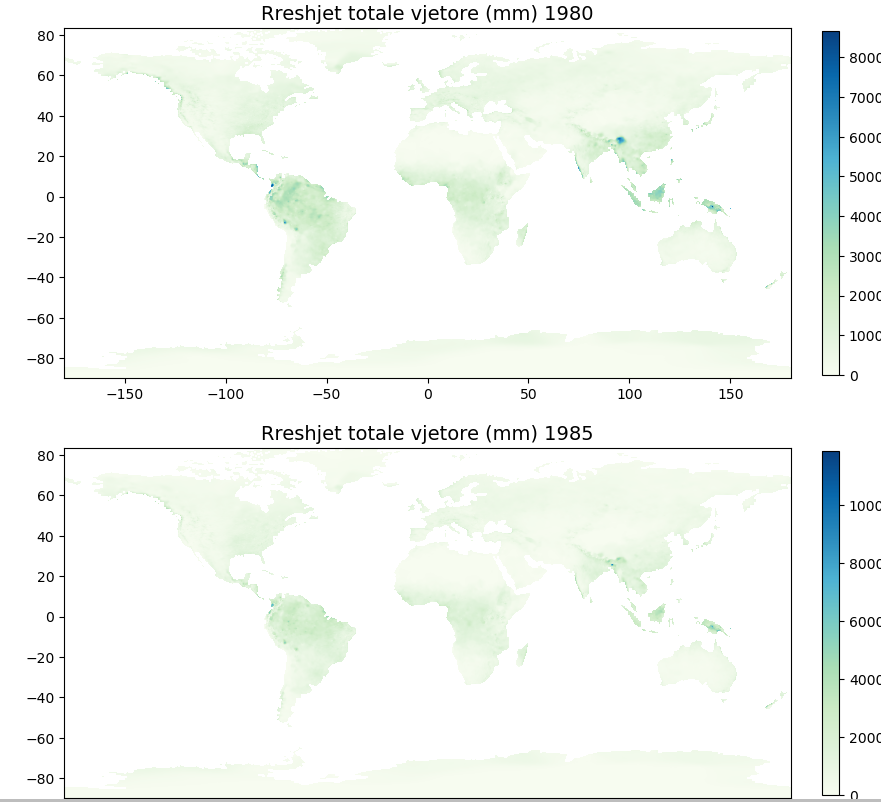
\includegraphics{./Figs/reshtotvjet.png}
\end{frame}

\begin{frame}{Ushtrimi 2}
\protect\hypertarget{ushtrimi-2}{}
\begin{itemize}
\item
  Duke përdorur veprimin e zbritjes nga algjebra e hartës, llogarisni
  dhe vizatoni diferencën e rasterit midis viteve 1980, 1990, 2000 dhe
  2010 (3 çifte).
\item
  Përdorni një cikël \textbf{for}.
\item
  Ripërdorni funksionin \textbf{plot\_raster}
\end{itemize}
\end{frame}

\begin{frame}[fragile]{Ndihmë}
\protect\hypertarget{ndihmuxeb}{}
\AddToHookNext{env/Highlighting/begin}{\tiny}

\begin{Shaded}
\begin{Highlighting}[]
\NormalTok{years }\OperatorTok{=}\NormalTok{ [}\DecValTok{1980}\NormalTok{,}\DecValTok{1990}\NormalTok{,}\DecValTok{2000}\NormalTok{,}\DecValTok{2010}\NormalTok{]}
\CommentTok{\# loop sipas viteve}
\ControlFlowTok{for}\NormalTok{ i }\KeywordTok{in} \BuiltInTok{range}\NormalTok{(}\BuiltInTok{len}\NormalTok{(years)}\OperatorTok{{-}}\DecValTok{1}\NormalTok{):}
\NormalTok{    year1 }\OperatorTok{=}\NormalTok{ years[i]}
\NormalTok{    year2 }\OperatorTok{=}\NormalTok{ years[i}\OperatorTok{+}\DecValTok{1}\NormalTok{]}
    \BuiltInTok{print}\NormalTok{(year1,year2)}
    \CommentTok{\# fusnin kodin ketu}
\end{Highlighting}
\end{Shaded}
\end{frame}

\begin{frame}[fragile]{Zgjidhje}
\protect\hypertarget{zgjidhje-3}{}
\AddToHookNext{env/Highlighting/begin}{\tiny}

\begin{Shaded}
\begin{Highlighting}[]
\NormalTok{years }\OperatorTok{=}\NormalTok{ [}\DecValTok{1980}\NormalTok{,}\DecValTok{1990}\NormalTok{,}\DecValTok{2000}\NormalTok{,}\DecValTok{2010}\NormalTok{]}
\CommentTok{\# loop sipas viteve}
\ControlFlowTok{for}\NormalTok{ i }\KeywordTok{in} \BuiltInTok{range}\NormalTok{(}\BuiltInTok{len}\NormalTok{(years)}\OperatorTok{{-}}\DecValTok{1}\NormalTok{):}
\NormalTok{    year1 }\OperatorTok{=}\NormalTok{ years[i]}
\NormalTok{    year2 }\OperatorTok{=}\NormalTok{ years[i}\OperatorTok{+}\DecValTok{1}\NormalTok{]}
    \BuiltInTok{print}\NormalTok{(}\StringTok{"Krahaso:"}\NormalTok{, year1, year2)}
    \CommentTok{\# Ngarkojme dy rastera per krahasim}
\NormalTok{    rast1 }\OperatorTok{=}\NormalTok{ rasterio.}\BuiltInTok{open}\NormalTok{(}\StringTok{\textquotesingle{}data/global\_precip\_raster{-}}\SpecialCharTok{\{\}}\StringTok{.asc\textquotesingle{}}\NormalTok{.}\BuiltInTok{format}\NormalTok{(year1), mask}\OperatorTok{=}\VariableTok{True}\NormalTok{)}
\NormalTok{    rast2 }\OperatorTok{=}\NormalTok{ rasterio.}\BuiltInTok{open}\NormalTok{(}\StringTok{\textquotesingle{}data/global\_precip\_raster{-}}\SpecialCharTok{\{\}}\StringTok{.asc\textquotesingle{}}\NormalTok{.}\BuiltInTok{format}\NormalTok{(year2), mask}\OperatorTok{=}\VariableTok{True}\NormalTok{)}
\NormalTok{    vals1 }\OperatorTok{=}\NormalTok{ rast1.read(}\DecValTok{1}\NormalTok{, masked}\OperatorTok{=}\VariableTok{True}\NormalTok{)}
\NormalTok{    vals2 }\OperatorTok{=}\NormalTok{ rast2.read(}\DecValTok{1}\NormalTok{, masked}\OperatorTok{=}\VariableTok{True}\NormalTok{)}
    \CommentTok{\# Llogarisim diferencen}
\NormalTok{    vals\_diff }\OperatorTok{=}\NormalTok{ vals2}\OperatorTok{{-}}\NormalTok{vals1}
    \BuiltInTok{print}\NormalTok{(}\StringTok{"Statistikat e diferences:"}\NormalTok{, vals\_diff.}\BuiltInTok{min}\NormalTok{(), }\BuiltInTok{round}\NormalTok{(vals\_diff.mean(),}\DecValTok{2}\NormalTok{), vals\_diff.}\BuiltInTok{max}\NormalTok{())}
    \CommentTok{\# Vizatoni diferencen}
\NormalTok{    plot\_raster(rast1, vals\_diff, }\StringTok{\textquotesingle{}Total precipitation change between }\SpecialCharTok{\{\}}\StringTok{ and }\SpecialCharTok{\{\}}\StringTok{\textquotesingle{}}\NormalTok{.}\BuiltInTok{format}\NormalTok{(year1,year2), }
            \StringTok{\textquotesingle{}Rreshje vjetore (mm)\textquotesingle{}}\NormalTok{, }\StringTok{\textquotesingle{}PuOr\textquotesingle{}}\NormalTok{, width}\OperatorTok{=}\DecValTok{10}\NormalTok{, height}\OperatorTok{=}\DecValTok{10}\NormalTok{, diverge\_zero}\OperatorTok{=}\VariableTok{True}\NormalTok{)}
\end{Highlighting}
\end{Shaded}
\end{frame}

\begin{frame}{Zgjidhje}
\protect\hypertarget{zgjidhje-4}{}
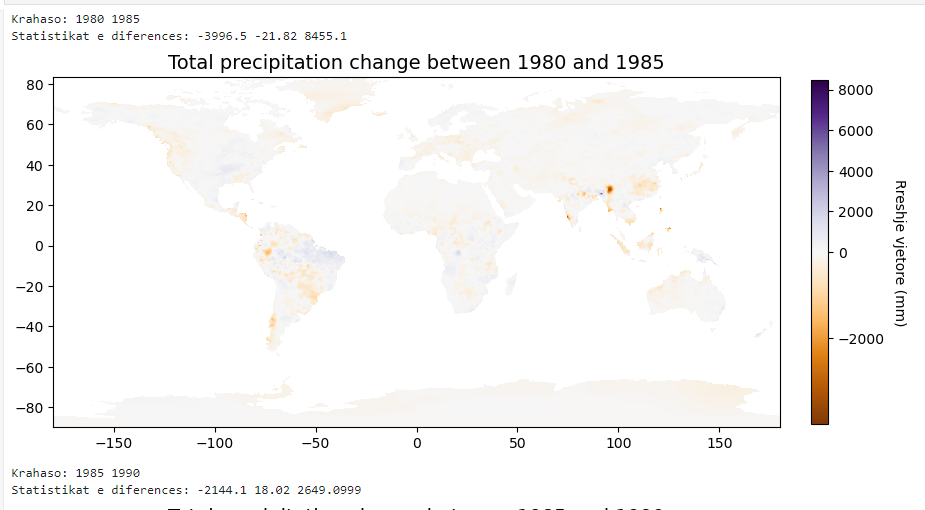
\includegraphics{./Figs/krahasim.png}
\end{frame}

\begin{frame}{Ushtrimi 3}
\protect\hypertarget{ushtrimi-3}{}
\begin{itemize}
\item
  Sa është sasia e reshjeve totale në çdo vend në vitin 2015?
\item
  Duke përdorur kufijtë e botës, përdorni statistikat zonale për t'iu
  përgjigjur kësaj pyetjeje.
\item
  Për çdo vend, llogarisni reshjet minimale, maksimale, mesatare,
  mediane dhe totale.
\item
  Ruani rezultatet në një tabelë CSV me një rresht për çdo vend dhe një
  kolonë për çdo statistikë përshkruese.
\end{itemize}
\end{frame}

\begin{frame}{Ushtrimi 3 (vazhdim)}
\protect\hypertarget{ushtrimi-3-vazhdim}{}
\begin{itemize}
\item
  Vini re se të dhënat e reshjeve janë shumë dhe rezultatet mund të
  paraqesin gabime të mëdha për vendet e vogla.
\item
  Përsëriteni analizën për vitin 1980: Duhet të bëni ndryshime minimale
  në kod.
\end{itemize}
\end{frame}

\begin{frame}[fragile]{Ndihmë}
\protect\hypertarget{ndihmuxeb-1}{}
\AddToHookNext{env/Highlighting/begin}{\tiny}

\begin{Shaded}
\begin{Highlighting}[]
\NormalTok{year }\OperatorTok{=} \DecValTok{2015}
\NormalTok{output\_file }\OperatorTok{=} \StringTok{\textquotesingle{}tmp/precipitation\_country\_stats\_\textquotesingle{}} \OperatorTok{+} \BuiltInTok{str}\NormalTok{(year) }\OperatorTok{+} \StringTok{\textquotesingle{}.csv\textquotesingle{}}
\BuiltInTok{print}\NormalTok{(output\_file)}

\CommentTok{\# futni kodin tuaj këtu}
\end{Highlighting}
\end{Shaded}
\end{frame}

\begin{frame}[fragile]{Zgjidhje}
\protect\hypertarget{zgjidhje-5}{}
\AddToHookNext{env/Highlighting/begin}{\tiny}

\begin{Shaded}
\begin{Highlighting}[]
\CommentTok{\# shkarkojmë hartën e botës}
\CommentTok{\# Shkarkoni gjithashtu kufijtë e vendeve}
\NormalTok{url\_boundaries }\OperatorTok{=} \StringTok{\textquotesingle{}https://github.com/endri81/instatgis/blob/master/data/gis4/natural\_earth\_world\_boundaries\_50m\_2018.geojson?raw=true\textquotesingle{}}
\NormalTok{file\_name\_boundaries }\OperatorTok{=} \StringTok{\textquotesingle{}data/natural\_earth\_world\_boundaries\_50m\_2018.geojson\textquotesingle{}}
\NormalTok{urllib.request.urlretrieve(url\_boundaries, file\_name\_boundaries)}
\end{Highlighting}
\end{Shaded}
\end{frame}

\begin{frame}[fragile]{Zgjidhje}
\protect\hypertarget{zgjidhje-6}{}
\AddToHookNext{env/Highlighting/begin}{\tiny}

\begin{Shaded}
\begin{Highlighting}[]
\CommentTok{\# Ngarkojmë kufijtë}
\NormalTok{countries\_df }\OperatorTok{=}\NormalTok{ gpd.read\_file(}\StringTok{\textquotesingle{}data/natural\_earth\_world\_boundaries\_50m\_2018.geojson\textquotesingle{}}\NormalTok{)}
\CommentTok{\# heqim vendet e panjohura}
\NormalTok{countries\_df }\OperatorTok{=}\NormalTok{ countries\_df[countries\_df.iso\_a3 }\OperatorTok{!=} \StringTok{\textquotesingle{}{-}99\textquotesingle{}}\NormalTok{]}
\BuiltInTok{print}\NormalTok{(}\BuiltInTok{len}\NormalTok{(countries\_df))}
\NormalTok{countries\_df.plot()}
\end{Highlighting}
\end{Shaded}
\end{frame}

\begin{frame}{Zgjidhje}
\protect\hypertarget{zgjidhje-7}{}
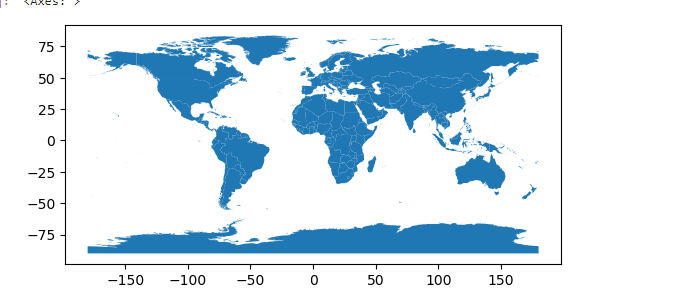
\includegraphics{./Figs/bota.png}
\end{frame}

\begin{frame}[fragile]{Zgjidhje}
\protect\hypertarget{zgjidhje-8}{}
\AddToHookNext{env/Highlighting/begin}{\tiny}

\begin{Shaded}
\begin{Highlighting}[]
\ImportTok{from}\NormalTok{ rasterstats }\ImportTok{import}\NormalTok{ zonal\_stats, gen\_zonal\_stats}

\ControlFlowTok{for}\NormalTok{ year }\KeywordTok{in}\NormalTok{ [}\DecValTok{1980}\NormalTok{, }\DecValTok{2015}\NormalTok{]:}
    \BuiltInTok{print}\NormalTok{(}\StringTok{"}\CharTok{\textbackslash{}n}\StringTok{Duke llogaritur statistikat zonale midis kufijve të vendeve të botës dhe reshjeve në }\SpecialCharTok{\{\}}\StringTok{..."}\NormalTok{.}\BuiltInTok{format}\NormalTok{(year))}
    \CommentTok{\# ngarkoni rasterin e reshjeve}
\NormalTok{    rast\_file }\OperatorTok{=} \StringTok{\textquotesingle{}data/global\_precip\_raster{-}}\SpecialCharTok{\{\}}\StringTok{.asc\textquotesingle{}}\NormalTok{.}\BuiltInTok{format}\NormalTok{(year)}
    \CommentTok{\# gjeneroni rrugën e skedarit të daljes}
\NormalTok{    output\_file }\OperatorTok{=} \StringTok{\textquotesingle{}tmp/precipitation\_country\_stats\_}\SpecialCharTok{\{\}}\StringTok{.csv\textquotesingle{}}\NormalTok{.}\BuiltInTok{format}\NormalTok{(year)}
    \CommentTok{\# llogarit statistikat zonale}
    \CommentTok{\# zgjidhni vetëm kolonat përkatëse nga countries\_df}
\NormalTok{    zon\_stats }\OperatorTok{=}\NormalTok{ zonal\_stats(countries\_df[[}\StringTok{\textquotesingle{}iso\_a3\textquotesingle{}}\NormalTok{,}\StringTok{\textquotesingle{}name\textquotesingle{}}\NormalTok{,}\StringTok{\textquotesingle{}geometry\textquotesingle{}}\NormalTok{]], rast\_file, }
\NormalTok{                            stats}\OperatorTok{=}\StringTok{"count min median mean max sum"}\NormalTok{, geojson\_out}\OperatorTok{=}\VariableTok{True}\NormalTok{)}
    \CommentTok{\# gjeneroni një kornizë të dhënash nga rezultatet e zonal\_stats (listë fjalorësh)}
\NormalTok{    stats\_gdf }\OperatorTok{=}\NormalTok{ gpd.GeoDataFrame.from\_features(zon\_stats)}
    \CommentTok{\# konverto nga geodataframe në dataframe, pasi nuk kemi nevojë për gjeometrinë}
\NormalTok{    stats\_df }\OperatorTok{=}\NormalTok{ pd.DataFrame(stats\_gdf.drop(columns}\OperatorTok{=}\StringTok{\textquotesingle{}geometry\textquotesingle{}}\NormalTok{))    }
    \CommentTok{\# hiqni vendet për të cilat nuk kemi vëzhgime}
\NormalTok{    stats\_df }\OperatorTok{=}\NormalTok{ stats\_df[stats\_df[}\StringTok{\textquotesingle{}count\textquotesingle{}}\NormalTok{] }\OperatorTok{\textgreater{}} \DecValTok{0}\NormalTok{]}
\NormalTok{    stats\_df }\OperatorTok{=}\NormalTok{ stats\_df.sort\_values(}\StringTok{\textquotesingle{}sum\textquotesingle{}}\NormalTok{)}
    \CommentTok{\# printoni statistikat}
    \BuiltInTok{print}\NormalTok{(stats\_df.describe())}
    \CommentTok{\# ruani rezultatet në skedar}
\NormalTok{    stats\_df.to\_csv(output\_file, index}\OperatorTok{=}\VariableTok{False}\NormalTok{)}
    \BuiltInTok{print}\NormalTok{(}\StringTok{"Rezultatet janë te"}\NormalTok{, output\_file)}
\end{Highlighting}
\end{Shaded}
\end{frame}

\begin{frame}{Zgjidhje}
\protect\hypertarget{zgjidhje-9}{}
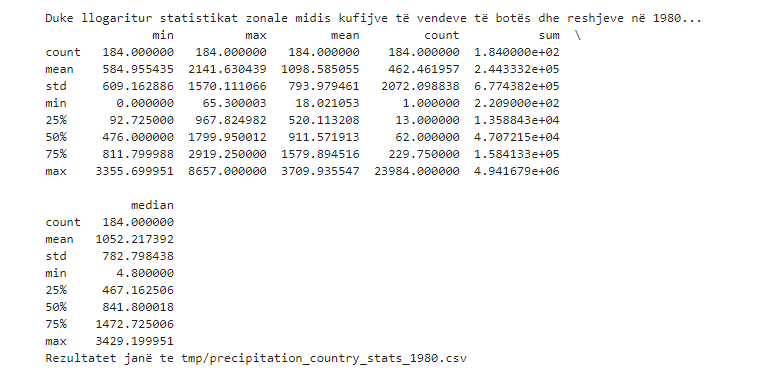
\includegraphics{./Figs/rezultate.png}
\end{frame}

\begin{frame}{Ushtrimi 4}
\protect\hypertarget{ushtrimi-4}{}
\begin{itemize}
\item
  Duke përdorur \textbf{.rank()}, gjeneroni renditje për vendet për sa i
  përket reshjeve të tyre (renditja 1 korrespondon me vendin më të
  lagësht).
\item
  Tregoni 10 vendet më të thata dhe më të lagështa në botë në vitin 1980
  dhe 2015.
\item
  A mund të vini re shumë ndryshime?
\end{itemize}
\end{frame}

\begin{frame}[fragile]{Ndihmë}
\protect\hypertarget{ndihmuxeb-2}{}
\AddToHookNext{env/Highlighting/begin}{\tiny}

\begin{Shaded}
\begin{Highlighting}[]
\NormalTok{years }\OperatorTok{=}\NormalTok{ [}\DecValTok{1980}\NormalTok{, }\DecValTok{2015}\NormalTok{]}
\ControlFlowTok{for}\NormalTok{ year }\KeywordTok{in}\NormalTok{ years:}
\NormalTok{    input\_stats\_file }\OperatorTok{=} \StringTok{\textquotesingle{}tmp/precipitation\_country\_stats\_\textquotesingle{}} \OperatorTok{+} \BuiltInTok{str}\NormalTok{(year) }\OperatorTok{+} \StringTok{\textquotesingle{}.csv\textquotesingle{}}
    \BuiltInTok{print}\NormalTok{(input\_stats\_file)}
    \CommentTok{\# ngarkoni skedarin dhe gjeneroni renditje}
\end{Highlighting}
\end{Shaded}
\end{frame}

\begin{frame}[fragile]{Zgjidhje}
\protect\hypertarget{zgjidhje-10}{}
\AddToHookNext{env/Highlighting/begin}{\tiny}

\begin{Shaded}
\begin{Highlighting}[]
\CommentTok{\# përcaktojmë "wet rank" bazuar në precipitimin mesatar.}
\NormalTok{years }\OperatorTok{=}\NormalTok{ [}\DecValTok{1980}\NormalTok{,}\DecValTok{2015}\NormalTok{]}

\CommentTok{\# bashkojmë statistikat në vite}
\NormalTok{wet\_rank\_df }\OperatorTok{=}\NormalTok{ countries\_df[[}\StringTok{\textquotesingle{}iso\_a3\textquotesingle{}}\NormalTok{,}\StringTok{\textquotesingle{}name\textquotesingle{}}\NormalTok{]]}

\ControlFlowTok{for}\NormalTok{ year }\KeywordTok{in}\NormalTok{ years:}
\NormalTok{    input\_stats\_file }\OperatorTok{=} \StringTok{\textquotesingle{}tmp/precipitation\_country\_stats\_\textquotesingle{}}\OperatorTok{+}\BuiltInTok{str}\NormalTok{(year)}\OperatorTok{+}\StringTok{\textquotesingle{}.csv\textquotesingle{}}
    \BuiltInTok{print}\NormalTok{(}\StringTok{"ranking"}\NormalTok{,input\_stats\_file)}
    \CommentTok{\# ngarkojme skedarin}
\NormalTok{    stats\_df }\OperatorTok{=}\NormalTok{ pd.read\_csv(input\_stats\_file)}
    \CommentTok{\# gjenerojme renditje}
\NormalTok{    rank\_field }\OperatorTok{=} \StringTok{\textquotesingle{}wet\_rank\_\textquotesingle{}}\OperatorTok{+}\BuiltInTok{str}\NormalTok{(year)}
\NormalTok{    stats\_df[rank\_field] }\OperatorTok{=}\NormalTok{ stats\_df[}\StringTok{\textquotesingle{}mean\textquotesingle{}}\NormalTok{].rank(ascending}\OperatorTok{=}\VariableTok{False}\NormalTok{)}
    \CommentTok{\# bashkojme rankimin me rezultatet finale}
\NormalTok{    wet\_rank\_df }\OperatorTok{=}\NormalTok{ wet\_rank\_df.merge(stats\_df[[}\StringTok{\textquotesingle{}iso\_a3\textquotesingle{}}\NormalTok{,rank\_field]], }
\NormalTok{                                    on}\OperatorTok{=}\StringTok{\textquotesingle{}iso\_a3\textquotesingle{}}\NormalTok{)}

\CommentTok{\# sort dhe ruaj rezultate}
\NormalTok{wet\_rank\_df[}\StringTok{\textquotesingle{}wet\_rank\_change\textquotesingle{}}\NormalTok{] }\OperatorTok{=}\NormalTok{ wet\_rank\_df[}\StringTok{\textquotesingle{}wet\_rank\_1980\textquotesingle{}}\NormalTok{]}\OperatorTok{{-}}\NormalTok{wet\_rank\_df[}\StringTok{\textquotesingle{}wet\_rank\_2015\textquotesingle{}}\NormalTok{]}
\NormalTok{wet\_rank\_df }\OperatorTok{=}\NormalTok{ wet\_rank\_df.sort\_values(}\StringTok{\textquotesingle{}wet\_rank\_2015\textquotesingle{}}\NormalTok{)}
\NormalTok{wet\_rank\_df.to\_csv(}\StringTok{\textquotesingle{}tmp/precipitation\_country\_stats.csv\textquotesingle{}}\NormalTok{, index}\OperatorTok{=}\VariableTok{False}\NormalTok{)}
\CommentTok{\# vendet më të lagështa 2015}
\NormalTok{wet\_rank\_df.head(}\DecValTok{10}\NormalTok{)}
\end{Highlighting}
\end{Shaded}
\end{frame}

\begin{frame}{Zgjidhje}
\protect\hypertarget{zgjidhje-11}{}
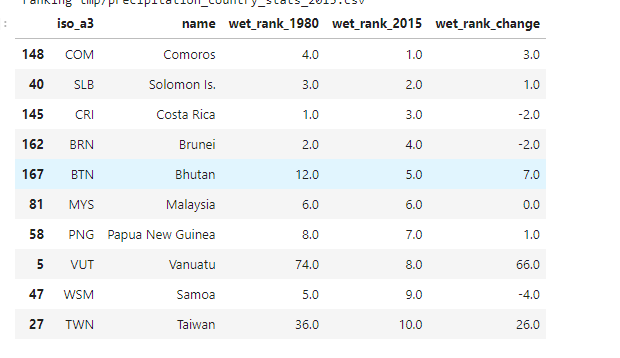
\includegraphics{./Figs/usht4.png}
\end{frame}

\begin{frame}[fragile]{Zgjidhje}
\protect\hypertarget{zgjidhje-12}{}
\AddToHookNext{env/Highlighting/begin}{\tiny}

\begin{Shaded}
\begin{Highlighting}[]
\CommentTok{\# vendet më të thata 2015}
\NormalTok{wet\_rank\_df.tail(}\DecValTok{10}\NormalTok{)}
\end{Highlighting}
\end{Shaded}
\end{frame}

\begin{frame}{Zgjidhje}
\protect\hypertarget{zgjidhje-13}{}
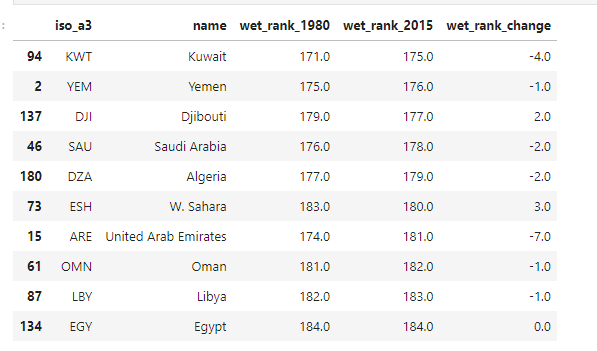
\includegraphics{./Figs/usht41.png}
\end{frame}

\begin{frame}[fragile]{Zgjidhje}
\protect\hypertarget{zgjidhje-14}{}
\AddToHookNext{env/Highlighting/begin}{\tiny}

\begin{Shaded}
\begin{Highlighting}[]
\CommentTok{\# vendet me ndryshime ekstreme në klasifikim}
\NormalTok{wet\_rank\_df[}\StringTok{\textquotesingle{}wet\_rank\_change\textquotesingle{}}\NormalTok{].hist()}
\end{Highlighting}
\end{Shaded}
\end{frame}

\begin{frame}{Zgjidhje}
\protect\hypertarget{zgjidhje-15}{}
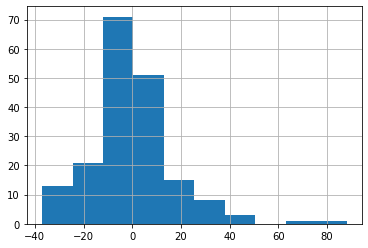
\includegraphics{./Figs/usht42.png}
\end{frame}

\begin{frame}[fragile]{Zgjidhje}
\protect\hypertarget{zgjidhje-16}{}
\AddToHookNext{env/Highlighting/begin}{\tiny}

\begin{Shaded}
\begin{Highlighting}[]
\CommentTok{\# vendet me ndryshime ekstreme }
\NormalTok{wet\_rank\_df }\OperatorTok{=}\NormalTok{ wet\_rank\_df.sort\_values(}\StringTok{\textquotesingle{}wet\_rank\_change\textquotesingle{}}\NormalTok{, ascending}\OperatorTok{=}\VariableTok{False}\NormalTok{)}
\CommentTok{\# Kontrollojmë diapazonin}
\NormalTok{extreme\_change\_df }\OperatorTok{=}\NormalTok{ wet\_rank\_df[}\OperatorTok{\textasciitilde{}}\NormalTok{wet\_rank\_df.wet\_rank\_change.between(}\OperatorTok{{-}}\DecValTok{20}\NormalTok{, }\DecValTok{20}\NormalTok{)]}
\NormalTok{extreme\_change\_df}
\end{Highlighting}
\end{Shaded}
\end{frame}

\begin{frame}{Zgjidhje}
\protect\hypertarget{zgjidhje-17}{}
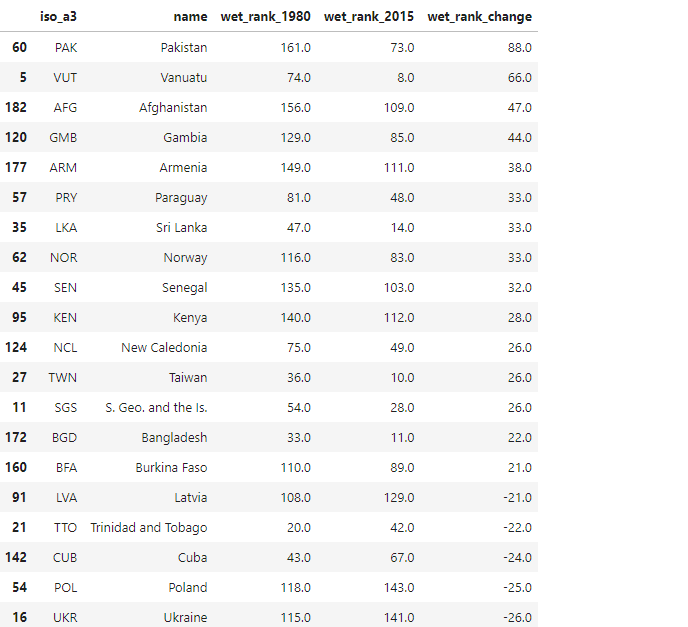
\includegraphics{./Figs/usht43.png}
\end{frame}

\begin{frame}{Ushtrimi 5}
\protect\hypertarget{ushtrimi-5}{}
\begin{itemize}
\item
  Duke përdorur \textbf{urllib.request.urlretrieve}, shkarkoni këtë
  dataset që përmban aeroportet globale.
\item
  Ngarkojeni në një dataframe gjeo me geopandas dhe printoni sa rreshta
  përmban.
\item
  Zgjidhni disa atribute prej saj, duke përfshirë emrin e aeroportit,
  kodin IATA të aeroportit, kodin e vendit, lartësinë dhe tipin.
\end{itemize}
\end{frame}

\begin{frame}[fragile]{Ndihmë}
\protect\hypertarget{ndihmuxeb-3}{}
\AddToHookNext{env/Highlighting/begin}{\tiny}

\begin{Shaded}
\begin{Highlighting}[]
\ImportTok{import}\NormalTok{ urllib.request}

\CommentTok{\# URL e azhurnuar për skedarin e aeroportit}
\NormalTok{airports\_url }\OperatorTok{=} \StringTok{\textquotesingle{}https://raw.githubusercontent.com/endri81/instatgis/master/data/gis4/airports\_2020.geojson\textquotesingle{}}

\CommentTok{\# Skedari lokal ku do të ruhet të dhënat}
\NormalTok{local\_file\_name }\OperatorTok{=} \StringTok{\textquotesingle{}data/airports\_2020.geojson\textquotesingle{}}
\BuiltInTok{print}\NormalTok{(local\_file\_name)}

\CommentTok{\# Shkarkoni skedarin nga URL{-}ja}
\NormalTok{urllib.request.urlretrieve(airports\_url, local\_file\_name)}

\CommentTok{\# futni kodin tuaj këtu}
\end{Highlighting}
\end{Shaded}
\end{frame}

\begin{frame}[fragile]{Zgjidhje}
\protect\hypertarget{zgjidhje-18}{}
\AddToHookNext{env/Highlighting/begin}{\tiny}

\begin{Shaded}
\begin{Highlighting}[]
\NormalTok{airports\_all\_df }\OperatorTok{=}\NormalTok{ gpd.read\_file(}\StringTok{\textquotesingle{}data/airports\_2020.geojson\textquotesingle{}}\NormalTok{)}
\BuiltInTok{print}\NormalTok{(}\StringTok{\textquotesingle{}n airports =\textquotesingle{}}\NormalTok{,}\BuiltInTok{len}\NormalTok{(airports\_all\_df))}
\BuiltInTok{print}\NormalTok{(airports\_all\_df.columns)}
\NormalTok{airports\_all\_df.sample(}\DecValTok{5}\NormalTok{)}
\end{Highlighting}
\end{Shaded}
\end{frame}

\begin{frame}{Zgjidhje}
\protect\hypertarget{zgjidhje-19}{}
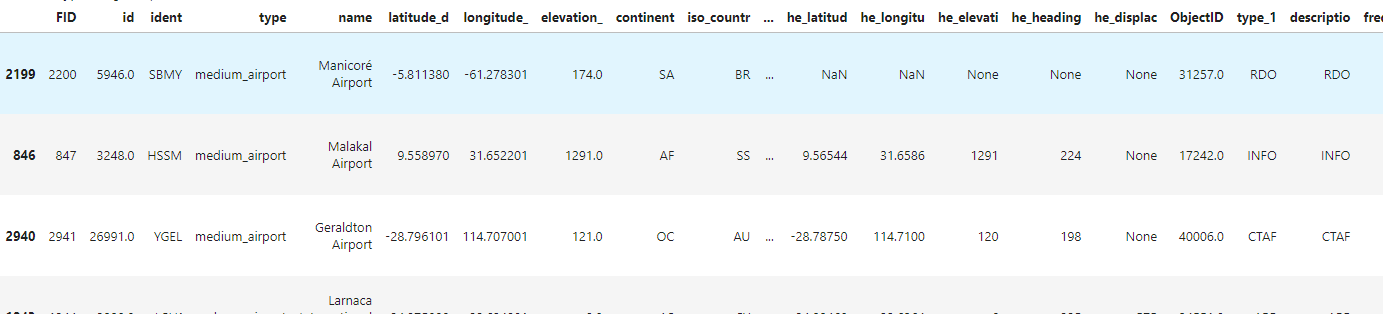
\includegraphics{./Figs/usht5.png}
\end{frame}

\begin{frame}[fragile]{Zgjidhje}
\protect\hypertarget{zgjidhje-20}{}
\AddToHookNext{env/Highlighting/begin}{\tiny}

\begin{Shaded}
\begin{Highlighting}[]
\NormalTok{airports\_df }\OperatorTok{=}\NormalTok{ airports\_all\_df[[}\StringTok{\textquotesingle{}id\textquotesingle{}}\NormalTok{,}\StringTok{\textquotesingle{}iata\_code\textquotesingle{}}\NormalTok{,}\StringTok{\textquotesingle{}name\textquotesingle{}}\NormalTok{,}\StringTok{\textquotesingle{}type\textquotesingle{}}\NormalTok{,}\StringTok{\textquotesingle{}iso\_countr\textquotesingle{}}\NormalTok{,}\StringTok{\textquotesingle{}elevation\_\textquotesingle{}}\NormalTok{,}\StringTok{\textquotesingle{}geometry\textquotesingle{}}\NormalTok{]]}
\CommentTok{\# rename elevation to show it is in feet}
\NormalTok{airports\_df }\OperatorTok{=}\NormalTok{ airports\_df.rename(columns}\OperatorTok{=}\NormalTok{\{}\StringTok{"elevation\_"}\NormalTok{: }\StringTok{"elevation\_ft"}\NormalTok{\})}
\CommentTok{\# show sample}
\NormalTok{airports\_df.sample(}\DecValTok{5}\NormalTok{)}
\end{Highlighting}
\end{Shaded}
\end{frame}

\begin{frame}{Zgjidhje}
\protect\hypertarget{zgjidhje-21}{}
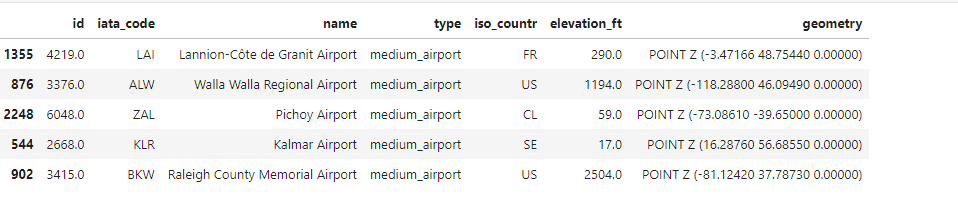
\includegraphics{./Figs/usht51.png}
\end{frame}

\begin{frame}{Ushtrimi 6}
\protect\hypertarget{ushtrimi-6}{}
\begin{itemize}
\item
  Analizoni densitetin e aeroporteve në botë.
\item
  Së pari, duke përdorur një histogram 2D me numër të ndryshëm të
  koshave (nga 20 në 100).
\item
  Bëni analizën për të gjitha aeroportet dhe vetëm për aeroportet e
  mëdha (type==`large\_airport').
\end{itemize}
\end{frame}

\begin{frame}[fragile]{Zgjidhje}
\protect\hypertarget{zgjidhje-22}{}
\AddToHookNext{env/Highlighting/begin}{\tiny}

\begin{Shaded}
\begin{Highlighting}[]
\CommentTok{\# ndryshojmë numrin e bin:}
\ControlFlowTok{for}\NormalTok{ bin\_n }\KeywordTok{in} \BuiltInTok{range}\NormalTok{(}\DecValTok{40}\NormalTok{,}\DecValTok{201}\NormalTok{,}\DecValTok{40}\NormalTok{):}
    \BuiltInTok{print}\NormalTok{(}\StringTok{"bin\_n"}\NormalTok{,bin\_n)}
    
    \CommentTok{\# ndryshojmë tipin}
    \ControlFlowTok{for}\NormalTok{ atype }\KeywordTok{in}\NormalTok{ [}\StringTok{\textquotesingle{}all\textquotesingle{}}\NormalTok{,}\StringTok{\textquotesingle{}large\_airport\textquotesingle{}}\NormalTok{]:}
\NormalTok{        df }\OperatorTok{=}\NormalTok{ airports\_df}
        \ControlFlowTok{if}\NormalTok{ atype }\OperatorTok{!=} \StringTok{\textquotesingle{}all\textquotesingle{}}\NormalTok{:}
\NormalTok{            df }\OperatorTok{=}\NormalTok{ airports\_df[airports\_df[}\StringTok{\textquotesingle{}type\textquotesingle{}}\NormalTok{] }\OperatorTok{==}\NormalTok{ atype]}
        \ControlFlowTok{assert} \BuiltInTok{len}\NormalTok{(df) }\OperatorTok{\textgreater{}} \DecValTok{0}
        \CommentTok{\# aeroportet e kërkuara janë në df}
\NormalTok{        h }\OperatorTok{=}\NormalTok{ plt.hist2d(df.geometry.x, df.geometry.y, bins}\OperatorTok{=}\NormalTok{bin\_n, density}\OperatorTok{=}\VariableTok{False}\NormalTok{)}
\NormalTok{        plt.colorbar(h[}\DecValTok{3}\NormalTok{])}
\NormalTok{        plt.title(}\StringTok{"2D histograma e aeroporteve (type=}\SpecialCharTok{\{\}}\StringTok{, bins=}\SpecialCharTok{\{\}}\StringTok{)"}\NormalTok{.}\BuiltInTok{format}\NormalTok{(atype, bin\_n))}
\NormalTok{        plt.show()}
\end{Highlighting}
\end{Shaded}
\end{frame}

\begin{frame}{Zgjidhje}
\protect\hypertarget{zgjidhje-23}{}
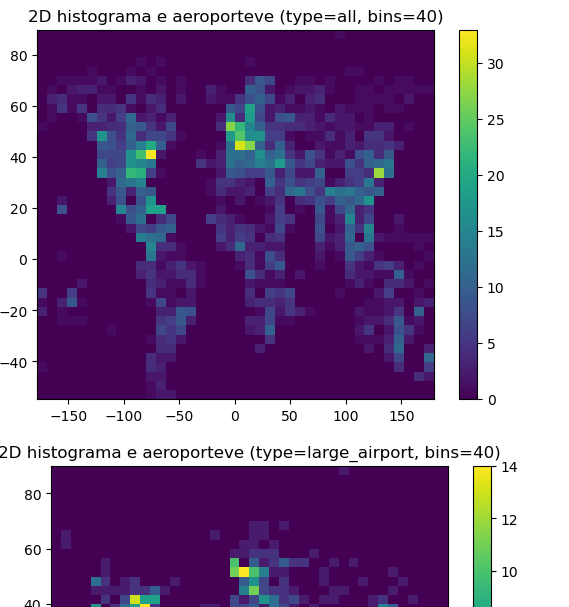
\includegraphics{./Figs/usht6.png}
\end{frame}

\begin{frame}{Ushtrimi 7}
\protect\hypertarget{ushtrimi-7}{}
\begin{itemize}
\item
  Gjeneroni KDE për aeroportet për Britaninë dhe SHBA-në duke ndryshuar
  gjerësinë e brezit në tre vlera të ndryshme që kapin shpërndarjen e
  aeroporteve në një mënyrë të përshtatshme.
\item
  Ku janë zonat më të dendura në botë? Ndani analizën midis të gjitha
  aeroporteve dhe vetëm aeroporteve të mëdha, duke minimizuar
  përsëritjen e kodit.
\end{itemize}
\end{frame}

\begin{frame}[fragile]{Zgjidhje}
\protect\hypertarget{zgjidhje-24}{}
\AddToHookNext{env/Highlighting/begin}{\tiny}

\begin{Shaded}
\begin{Highlighting}[]
\ImportTok{import}\NormalTok{ geoplot}
\ImportTok{import}\NormalTok{ matplotlib.pyplot }\ImportTok{as}\NormalTok{ plt}

\CommentTok{\# Për secilin vend, \textquotesingle{}US\textquotesingle{} dhe \textquotesingle{}GB\textquotesingle{}}
\ControlFlowTok{for}\NormalTok{ country }\KeywordTok{in}\NormalTok{ [}\StringTok{\textquotesingle{}US\textquotesingle{}}\NormalTok{, }\StringTok{\textquotesingle{}GB\textquotesingle{}}\NormalTok{]:}
    \CommentTok{\# zgjidh aeroportet në adf}
\NormalTok{    adf }\OperatorTok{=}\NormalTok{ airports\_df[airports\_df[}\StringTok{\textquotesingle{}iso\_countr\textquotesingle{}}\NormalTok{] }\OperatorTok{==}\NormalTok{ country]}
\NormalTok{    cdf }\OperatorTok{=}\NormalTok{ countries\_df[countries\_df[}\StringTok{\textquotesingle{}iso\_a2\textquotesingle{}}\NormalTok{] }\OperatorTok{==}\NormalTok{ country]}
    
    \CommentTok{\# nëse vendi është \textquotesingle{}GB\textquotesingle{}, largoni një aeroport RAF në Qipro}
    \ControlFlowTok{if}\NormalTok{ country }\OperatorTok{==} \StringTok{\textquotesingle{}GB\textquotesingle{}}\NormalTok{:}
\NormalTok{        adf }\OperatorTok{=}\NormalTok{ adf[adf[}\StringTok{\textquotesingle{}iata\_code\textquotesingle{}}\NormalTok{] }\OperatorTok{!=} \StringTok{\textquotesingle{}AKT\textquotesingle{}}\NormalTok{]}
    
    \CommentTok{\# sigurohuni që të dhënat e vendit dhe aeroportit të mos jenë bosh}
    \ControlFlowTok{assert} \BuiltInTok{len}\NormalTok{(cdf) }\OperatorTok{\textgreater{}} \DecValTok{0}
    \ControlFlowTok{assert} \BuiltInTok{len}\NormalTok{(adf) }\OperatorTok{\textgreater{}} \DecValTok{0}

    \CommentTok{\# ndryshoni bandwidth}
    \ControlFlowTok{for}\NormalTok{ bandwidth }\KeywordTok{in}\NormalTok{ [}\FloatTok{.01}\NormalTok{, }\FloatTok{.05}\NormalTok{, }\FloatTok{.1}\NormalTok{]:}
\NormalTok{        title }\OperatorTok{=} \StringTok{\textquotesingle{}KDE për aeroportet (vendi=}\SpecialCharTok{\{\}}\StringTok{, bandwidth=}\SpecialCharTok{\{\}}\StringTok{)\textquotesingle{}}\NormalTok{.}\BuiltInTok{format}\NormalTok{(country, bandwidth)}
\NormalTok{        ax }\OperatorTok{=}\NormalTok{ geoplot.kdeplot(adf, shade}\OperatorTok{=}\VariableTok{False}\NormalTok{, bw}\OperatorTok{=}\NormalTok{bandwidth, figsize}\OperatorTok{=}\NormalTok{(}\DecValTok{12}\NormalTok{, }\DecValTok{12}\NormalTok{), alpha}\OperatorTok{=}\FloatTok{.5}\NormalTok{)}
        
        \CommentTok{\# shtoni vijën bregdetare}
\NormalTok{        cdf.plot(ax}\OperatorTok{=}\NormalTok{ax, color}\OperatorTok{=}\StringTok{\textquotesingle{}lightgray\textquotesingle{}}\NormalTok{, edgecolor}\OperatorTok{=}\StringTok{"none"}\NormalTok{, linewidth}\OperatorTok{=}\FloatTok{.5}\NormalTok{)}
        
        \CommentTok{\# shtoni titullin}
\NormalTok{        plt.title(title, fontsize}\OperatorTok{=}\DecValTok{18}\NormalTok{)}
        
        \CommentTok{\# shfaqni figurën}
\NormalTok{        plt.show()}
\end{Highlighting}
\end{Shaded}
\end{frame}

\begin{frame}{Zgjidhje}
\protect\hypertarget{zgjidhje-25}{}
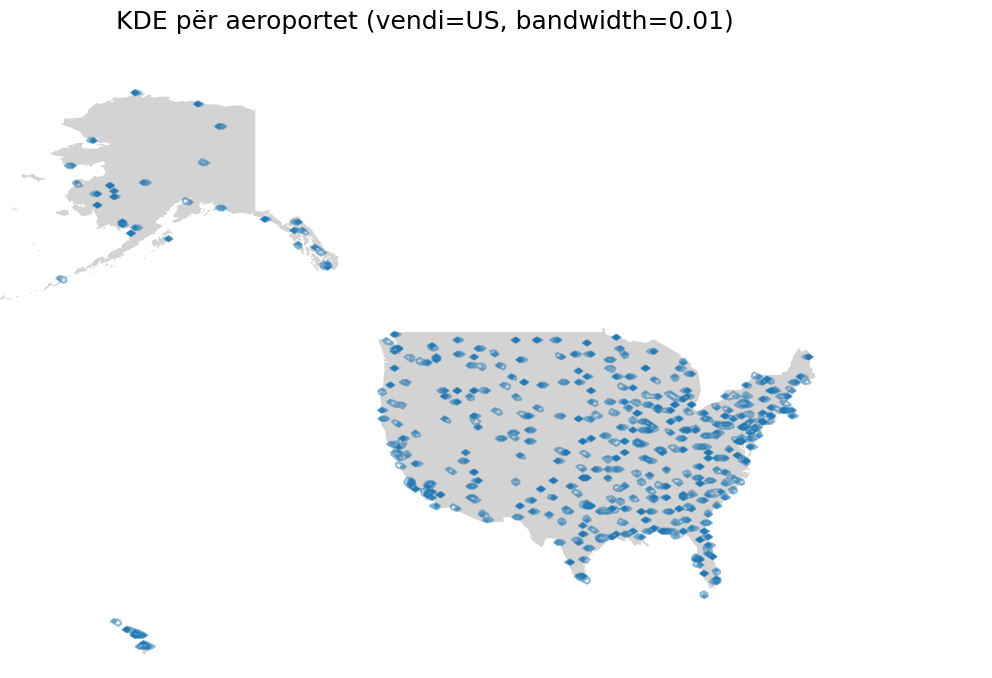
\includegraphics{./Figs/usht7.png}
\end{frame}

\end{document}
